%!TEX root = ../thesis.tex
%*******************************************************************************
%****************************** Second Chapter *********************************
%*******************************************************************************

\chapter{Multi-task Learning Mitigation Strategy}
\label{ch2}

\ifpdf
    \graphicspath{{Chapter2/Figs/Raster/}{Chapter2/Figs/PDF/}{Chapter2/Figs/}}
\else
    \graphicspath{{Chapter2/Figs/Vector/}{Chapter2/Figs/}}
\fi

In this chapter, I present the social robotics use cases that serve as the primary empirical reference for this study. Furthermore, I revisit established ML frameworks to formalize an architecture for culturally competent ML, together with the definition of appropriate evaluation metrics. I then propose a mitigation strategy based on Multi-Task Learning (MTL), designed to address cultural bias in robotic perception.

The subsequent section presents the empirical evaluations conducted using the methodologies introduced in this chapter. The analysis begins with a formal characterization of the main objective: quantifying the cultural competence of ML models under conditions of significant data sparsity and under-representation.

Subsequent sections assess the cultural competence of baseline ML models under varying degrees of cultural under-representation. Finally, a discussion section summarizes the findings.
%
\section{Case Studies}
\label{ch2:sec:data}

It is necessary to reiterate the premise established in Section~\ref{ch1:sec:sota}: the definition of the case studies is necessitated by the current absence of standardized benchmark datasets dedicated to cultural competence in SR. 
This lack of established infrastructure currently prevents researchers from conducting rigorous comparative evaluations of proposed methodologies.

In this research, two distinct image recognition tasks are developed to evaluate cultural competence in robotic perception: the recognition of lighting states (LAMP) and the detection of floor coverings (CARPET).

The LAMP task is formulated as a binary classification problem designed to determine whether a lamp is in an active (on) or inactive (off) state. The dataset for this task comprises images sourced from three distinct cultural contexts: Chinese, French, and Turkish. 
From a functional perspective, this task exemplifies the role of SRs in monitoring the domestic environment to detect anomalous nighttime behaviors among older adults or individuals with cognitive impairments. 
Similar applications include the state estimation of critical household infrastructure, such as determining whether refrigerators, entrance doors, windows, or water fixtures remain open or closed.

The CARPET task is likewise established as a binary classification problem, focused on identifying the presence or absence of a carpet within a domestic interior. 
This dataset incorporates visual data from Indian, Scandinavian, and Japanese cultural contexts. 
This task underscores the utility of SAR in environmental risk assessment; specifically, the detection of carpets is vital for mitigating fall risks and preventing accidents, thereby enhancing the autonomous mobility and physical safety of vulnerable populations.

From a technological standpoint, the selection of these specific image classification tasks and cultural domains was informed by several critical factors.

First, there is a direct alignment between these tasks and the fundamental challenges of ML in SR. 
Lamps and carpets exhibit distinct, culturally-mediated morphological features that are highly recognizable within the selected regions, providing a robust basis for evaluating cultural adaptation.

Second, these tasks are calibrated to a mid-level complexity; they are sufficiently non-trivial to require sophisticated analysis but remain tractable enough to permit the comparative evaluation of diverse ML paradigms, ranging from shallow architectures to deep neural networks. 
It is hypothesized that deep models will demonstrate significantly higher performance benchmarks compared to their shallow counterparts.

Finally, the inherent difficulty of these problems does not necessitate the acquisition of massive datasets comprising millions of samples—a scale of data that is frequently prohibitive to retrieve and annotate. 
This logistical constraint underscores a central premise of this research: for minority cultures, the conventional "big data" solution of simply increasing the sample size is often unfeasible, necessitating the development of more sophisticated algorithmic mitigation strategies.

The two datasets were curated following a rigorous protocol designed to minimize manual intervention while maintaining the high standards of quality necessary for a specialized research corpus. 
Although automation was prioritized, selective manual oversight was integrated to ensure data integrity and relevance. 
The acquisition process is delineated as follows:Initial data retrieval was conducted using the Selenium framework\footnote{\url{www.selenium.dev}} to automate search queries on Google Images\footnote{\url{www.images.google.com}}. 
For each primary query, the first $M$ images were downloaded; subsequently, the first $N$ "visually similar" images were retrieved for each of these $M$ results to expand the breadth of the dataset. The specific values for $M$ and $N$, alongside the corresponding culture-specific search queries, are detailed in Table~\ref{ch2:tab:casestudy:1}.To refine the automated results, a keyword-based filtration step was implemented, where the metadata and descriptions of all retrieved images were audited for the presence of specific identifiers. 
These culture-specific keywords are documented in Table~\ref{ch2:tab:casestudy:2}.
Following this automated pipeline, a manual visual inspection was performed to identify and expunge low-quality entries, including images with significant occlusion, superimposed text, or watermarks. 
For the LAMP dataset specifically, an additional preprocessing step was executed to isolate the primary object from its environmental context. 
Background removal was performed using the Remove.bg API\footnote{\url{www.remove.bg}}, followed by a manual quality assurance check to verify the accuracy of the segmentation masks.

The application of the aforementioned protocols resulted in the final datasets summarized in Table~\ref{ch2:tab:casestudy:3}, which have been made publicly available to the research community\footnote{\url{https://github.com/lucaoneto/CulturalCompetentML}}. 
To provide visual clarity regarding the dataset's composition, representative samples for each cultural context and target class are illustrated in Figure~\ref{ch2:fig:casestudy:1} for the LAMP dataset and Figure~\ref{ch2:fig:casestudy:2} for the CARPET dataset.

%
\begin{table*}
\footnotesize
\centering
\setlength{\tabcolsep}{0.1cm}
\renewcommand{\arraystretch}{1.5}
\begin{tabular}{l|p{12.5cm}|c|c}
\toprule
\textbf{Culture} &  \textbf{Queries} & $M$ & $N$  \\
\midrule
\multicolumn{4}{c}{\textbf{LAMP dataset}}\\
\midrule
Chinese & ``Chinese lamp'', ``Chinese table lamp'' & 50 & 80  \\
\hline
French &``French lamp'', ``French table lamp'', ``French lamps'' & 50 & 80  \\
\hline
Turkish & ``Mosaic Turkish lamp'', ``Turkish lamp'' & 50 & 80 \\
\midrule
\multicolumn{4}{c}{\textbf{CARPET dataset}}\\
\midrule
Indian & ``Traditional Indian house with carpet'', ``Traditional Indian house floor'', ``Traditional Indian house interior'', ``Antique Indian house interior'' & 60 & 90 \\
\hline
Japanese & ``Traditional Japanese house with carpet'', ``Traditional Japanese house floor'', ``Traditional Japanese house interior'', ``Antique Japanese house interior'' & 60 & 90 \\
\hline
Scandinavian & ``Traditional Scandinavian house with carpet'', ``Traditional Scandinavian house floor'', ``Traditional Scandinavian house interior'', ``Antique Scandinavian house interior'' & 60 & 90 \\
\bottomrule
\end{tabular}
\caption{Adopted queries, $M$, and $N$ exploited during the data collection for the LAMP and CARPET datasets.}
\label{ch2:tab:casestudy:1}
\end{table*}
%
\begin{table*}
\footnotesize
\centering
\setlength{\tabcolsep}{0.1cm}
\renewcommand{\arraystretch}{1.5}
\begin{tabular}{l|l|p{12cm}}
\toprule
\textbf{Dataset} & \textbf{Culture} & \textbf{Keywords} \\
\midrule
\multirow{6}{*}{LAMP} & Chinese & chinese, lamp, china ,lamps, oriental, asian, antique, porcelain, bouillotte, cinese, cinesi, lampada, lampade, lantern, lanterns, lanterna, lanterne, orientale, orientali, asiatica, asiatiche, asiatico, antico, porcellana\\
\hhline{~--}
& French & french, lamp, france, lamps, european, art deco, liberty, bat-jour, bouillotte, francese, francesi, lampada, lampade, europea, europee\\
\hhline{~--}
& Turkish & turkish, turkey, lamp, lamps, traditional, arabic, arabian, oriental, table, mosaic, antique, turca, turche, lampada, lampade,tradizionale, araba, orientale, tavolo,  antico\\
\midrule
\multirow{3}{*}{CARPET} & Indian &  indian, home, decor, carpet, indiano, casa, traditional, rug, rugs, tappeto, tappeti \\
\hhline{~--}
& Japanese & japanese, home, decor, carpet, giapponese, casa, traditional, rug, rugs, tappeto, tappeti\\
\hhline{~--}
& Scandinavian & scandinavian, home, decor, carpet, scandinavo, casa, traditional, rug, rugs, tappeto, tappeti \\
\bottomrule
\end{tabular}
\caption{Adopted keywords exploited during the data collection for the LAMP and CARPET datasets.}
\label{ch2:tab:casestudy:2}
\end{table*}
%
\begin{table}
\footnotesize
\centering
\setlength{\tabcolsep}{0.1cm}
\renewcommand{\arraystretch}{1.5}
\begin{tabular}{|l|l|c|c|}
\toprule
\textbf{Dataset} & \textbf{Culture} & \textbf{Class} & \textbf{n° Images} \\
\midrule
\multirow{6}{*}{LAMP} & \multirow{2}{*}{Chinese} & On & 1013\\
\hhline{~~-}
& & Off & 1058\\
\hhline{~--}
& \multirow{2}{*}{French} & On & 1019\\
\hhline{~~-}
& & Off & 1022\\
\hhline{~--}
& \multirow{2}{*}{Turkish} & On & 1020\\
\hhline{~~-}
& & Off & 1001\\
\midrule
\multirow{6}{*}{CARPET} & \multirow{2}{*}{Indian} & Present & 1178\\
\hhline{~~-}
& & Absent & 1065\\
\hhline{~--}
& \multirow{2}{*}{Japanese} & Present & 1005\\
\hhline{~~-}
& & Absent & 1250\\
\hhline{~--}
& \multirow{2}{*}{Scandinavian} & Present & 1394\\
\hhline{~~-}
& & Absent & 1031\\
\bottomrule
\end{tabular}
\caption{Summary of the final LAMP and CARPET collected datasets.}
\label{ch2:tab:casestudy:3}
\end{table}
%
\begin{figure*}
\centering
\begin{subfigure}[b]{0.3\columnwidth}
\centering

\includegraphics[width=\columnwidth]{LCN.jpg}
\caption{Chinese - On.}
\end{subfigure}
\begin{subfigure}[b]{0.3\columnwidth}
\centering
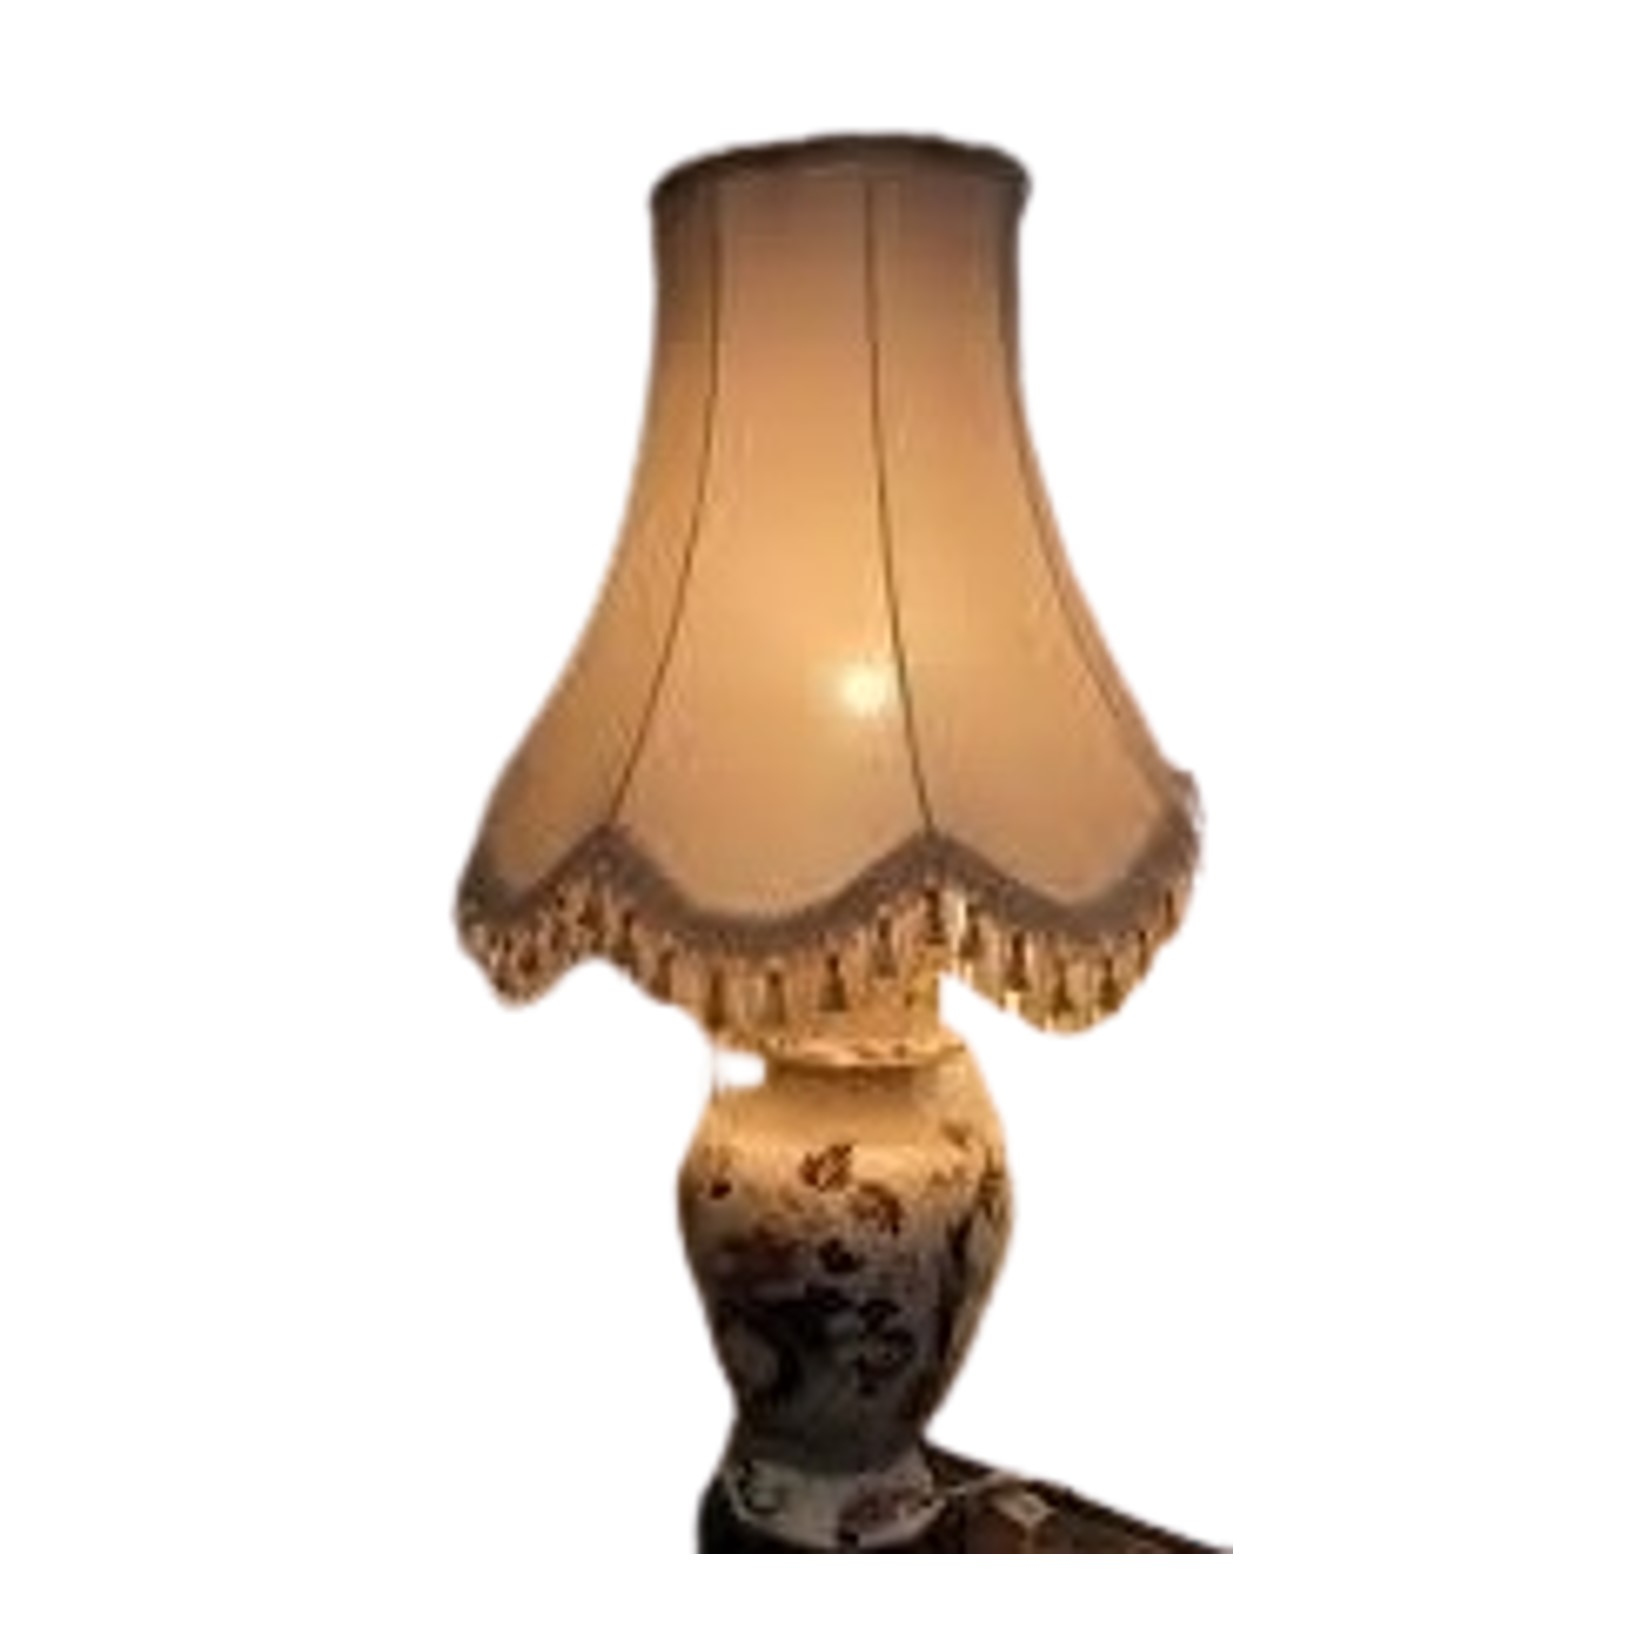
\includegraphics[width=\columnwidth]{LFN.jpg}
\caption{French - On.}
\end{subfigure}
\begin{subfigure}[b]{0.3\columnwidth}
\centering

\includegraphics[width=\columnwidth]{LTN.jpg}
\caption{Turkish - On.}
\end{subfigure} \\
\begin{subfigure}[b]{0.3\columnwidth}
\centering

\includegraphics[width=\columnwidth]{LCF.jpg}
\caption{Chinese - Off.}
\end{subfigure}
\begin{subfigure}[b]{0.3\columnwidth}
\centering

\includegraphics[width=\columnwidth]{LFF.jpg}
\caption{French - Off.}
\end{subfigure}
\begin{subfigure}[b]{0.3\columnwidth}
\centering
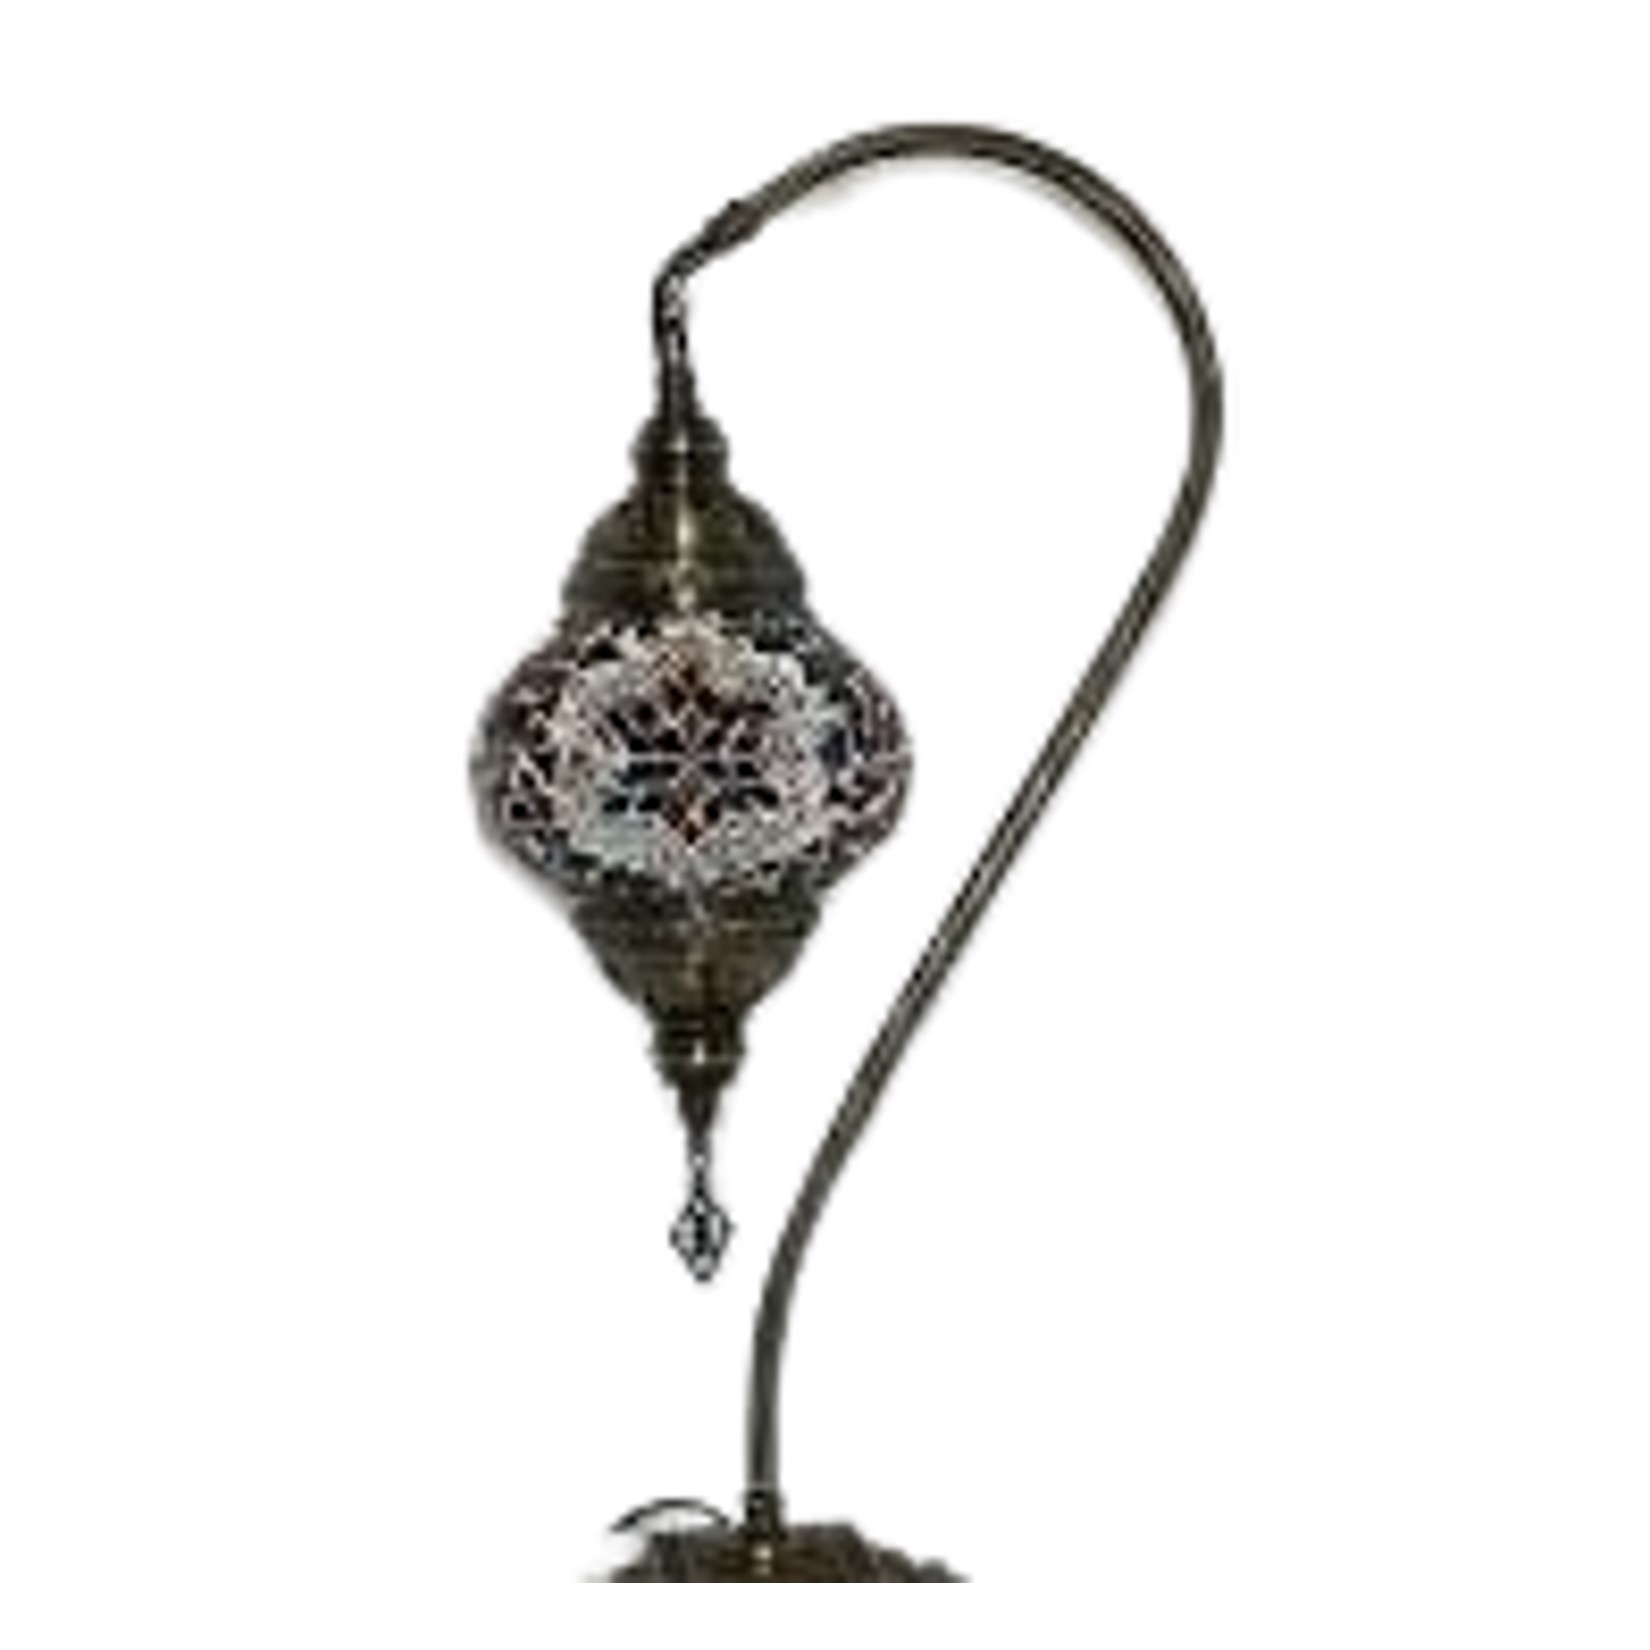
\includegraphics[width=\columnwidth]{LTF.jpg}
\caption{Turkish - Off.}
\end{subfigure}
\caption{Samples from the LAMP dataset.}
\label{ch2:fig:casestudy:1}
\end{figure*}
%
\begin{figure*}
\centering
\begin{subfigure}[b]{0.3\columnwidth}
\centering
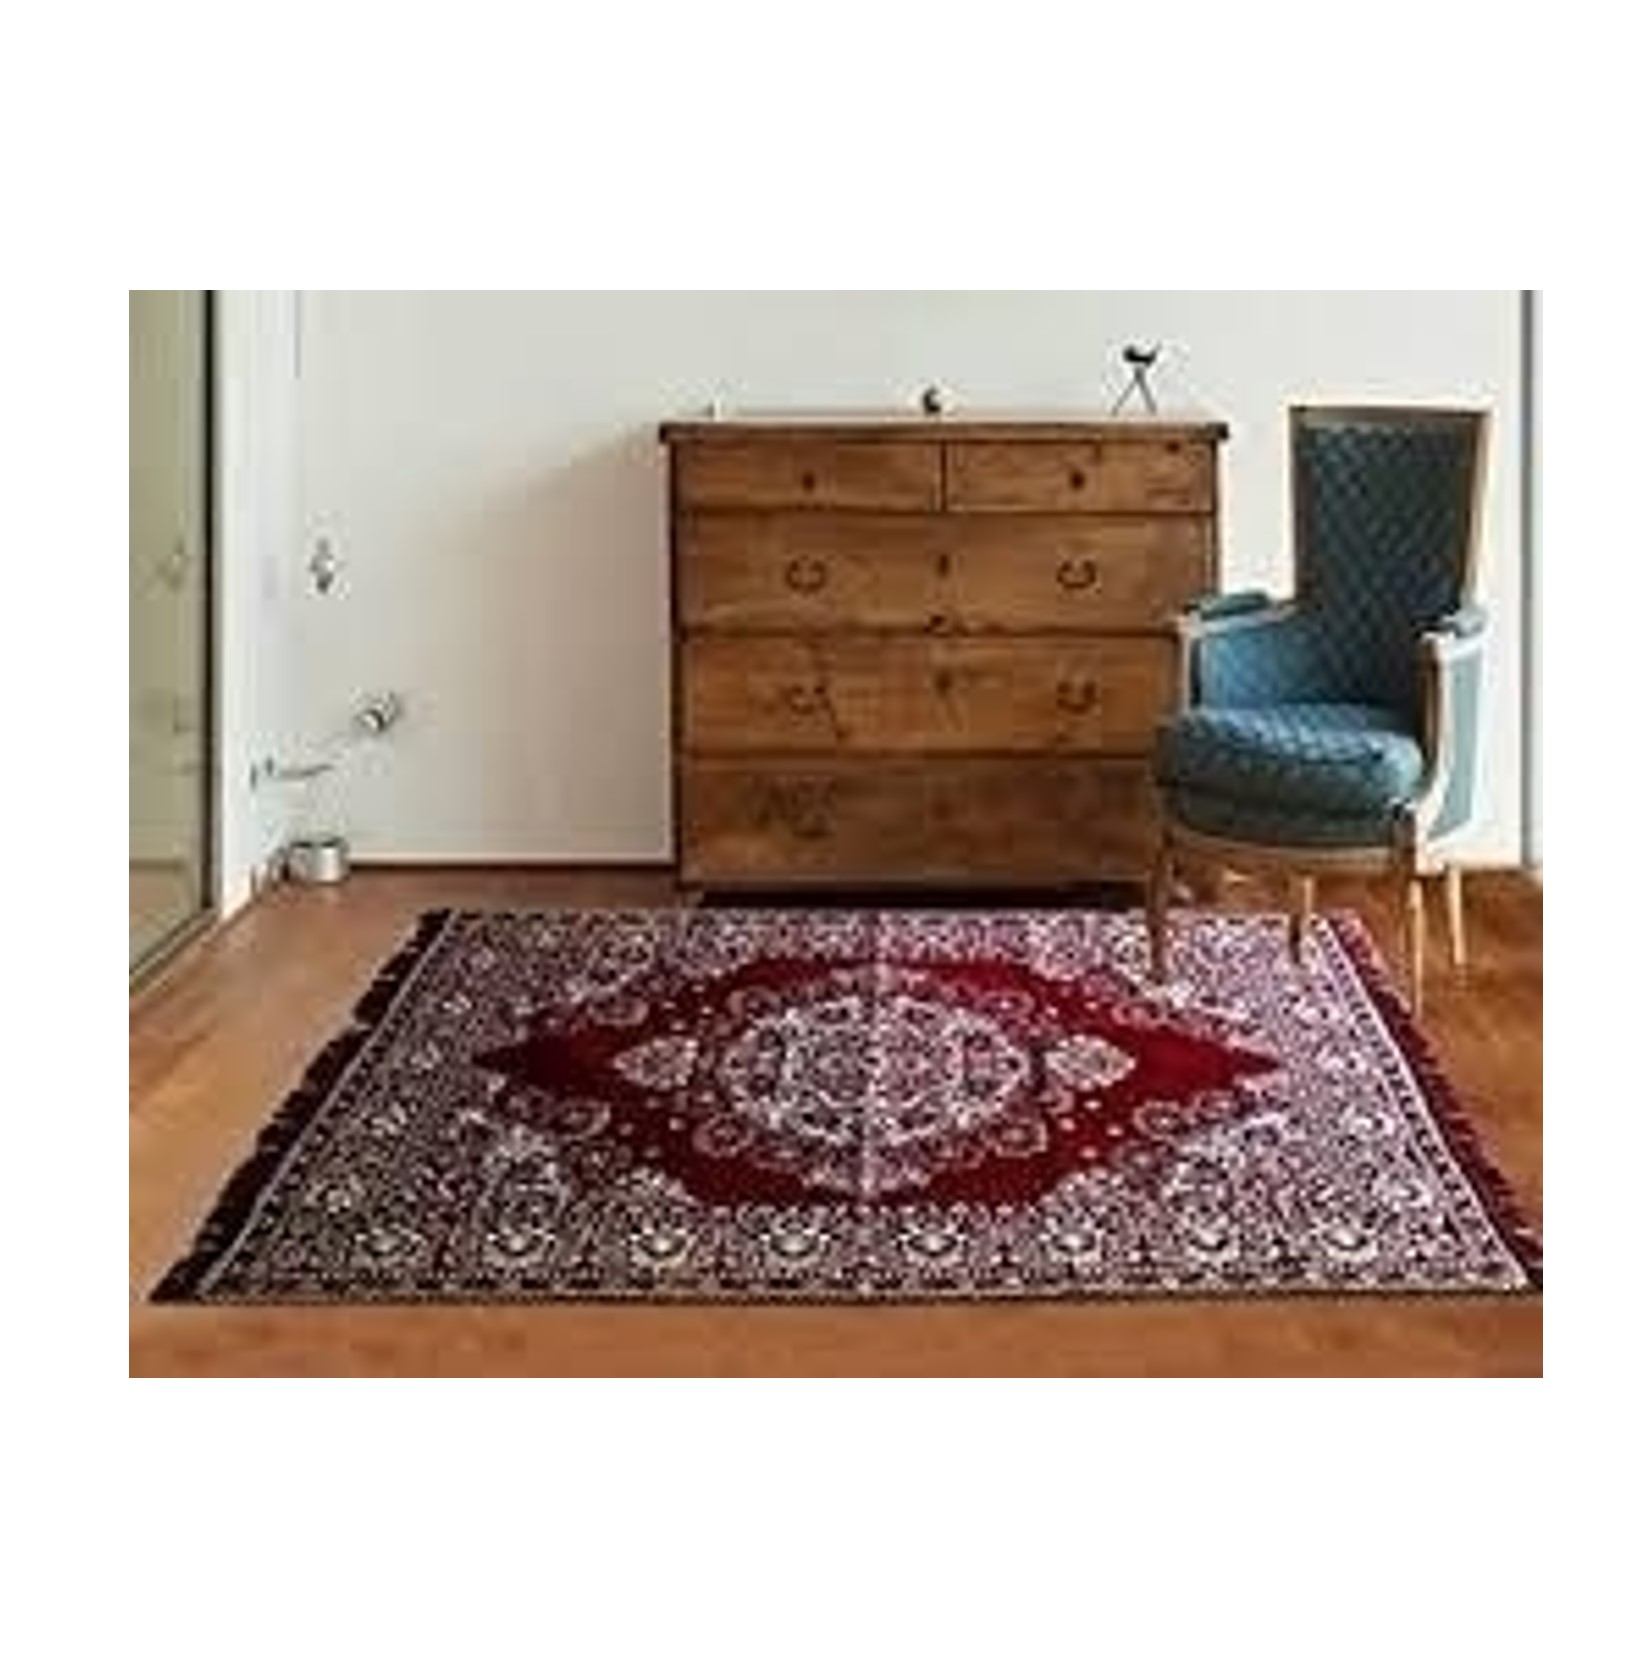
\includegraphics[width=\columnwidth]{CIP.jpg}
\caption{Indian - Present.}
\end{subfigure}
\begin{subfigure}[b]{0.3\columnwidth}
\centering
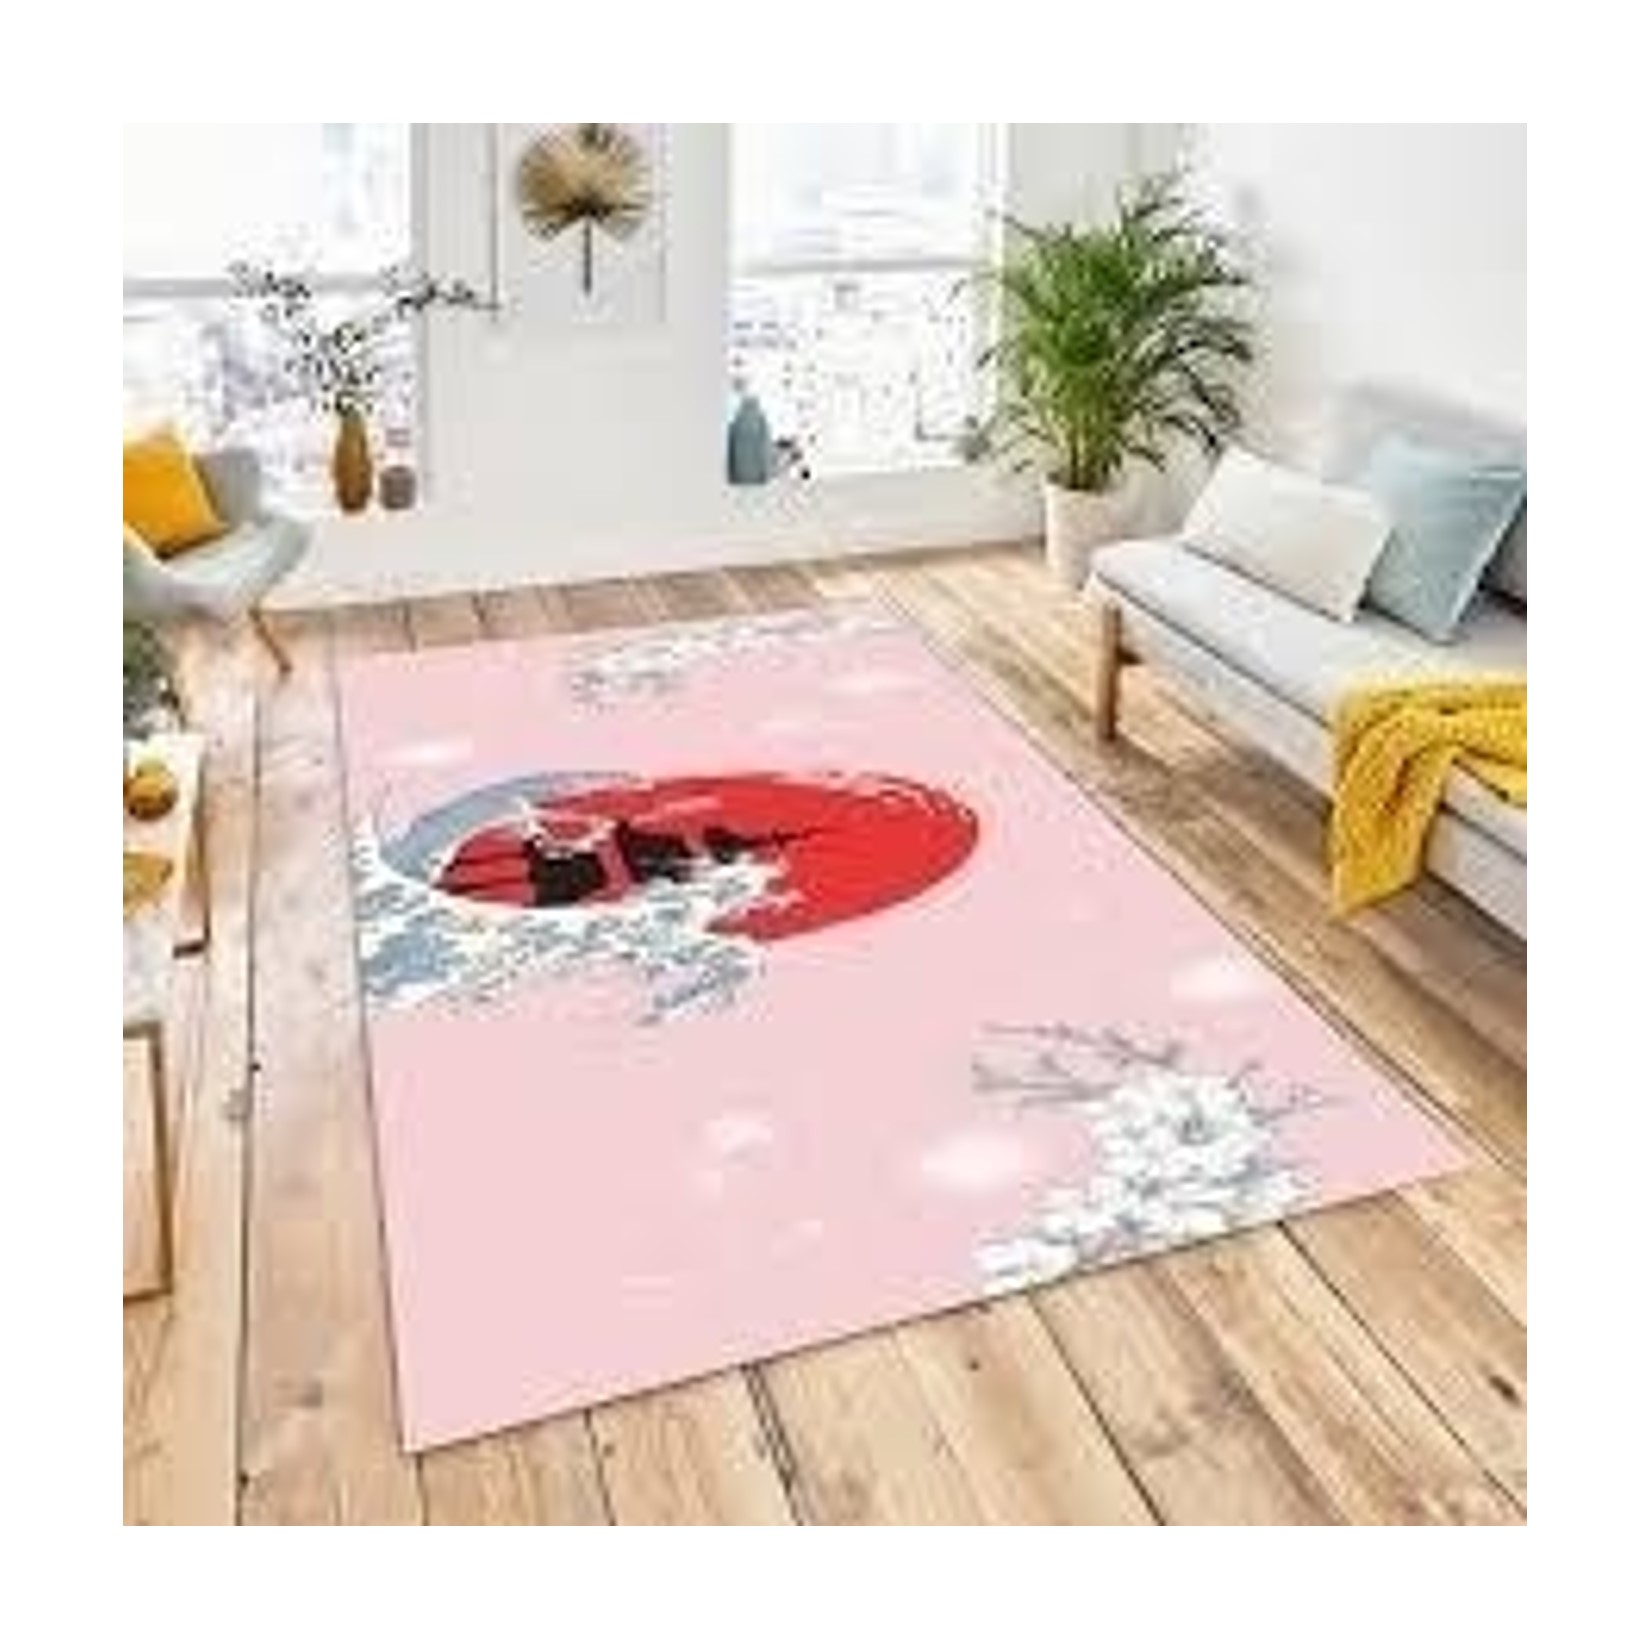
\includegraphics[width=\columnwidth]{CJP.jpg}
\caption{Japanese - Present.}
\end{subfigure}
\begin{subfigure}[b]{0.3\columnwidth}
\centering

\includegraphics[width=\columnwidth]{CSP.jpg}
\caption{Scandinavian - Present.}
\end{subfigure} \\
\begin{subfigure}[b]{0.3\columnwidth}
\centering

\includegraphics[width=\columnwidth]{CIA.jpg}
\caption{Indian - Absent.}
\end{subfigure}
\begin{subfigure}[b]{0.3\columnwidth}
\centering
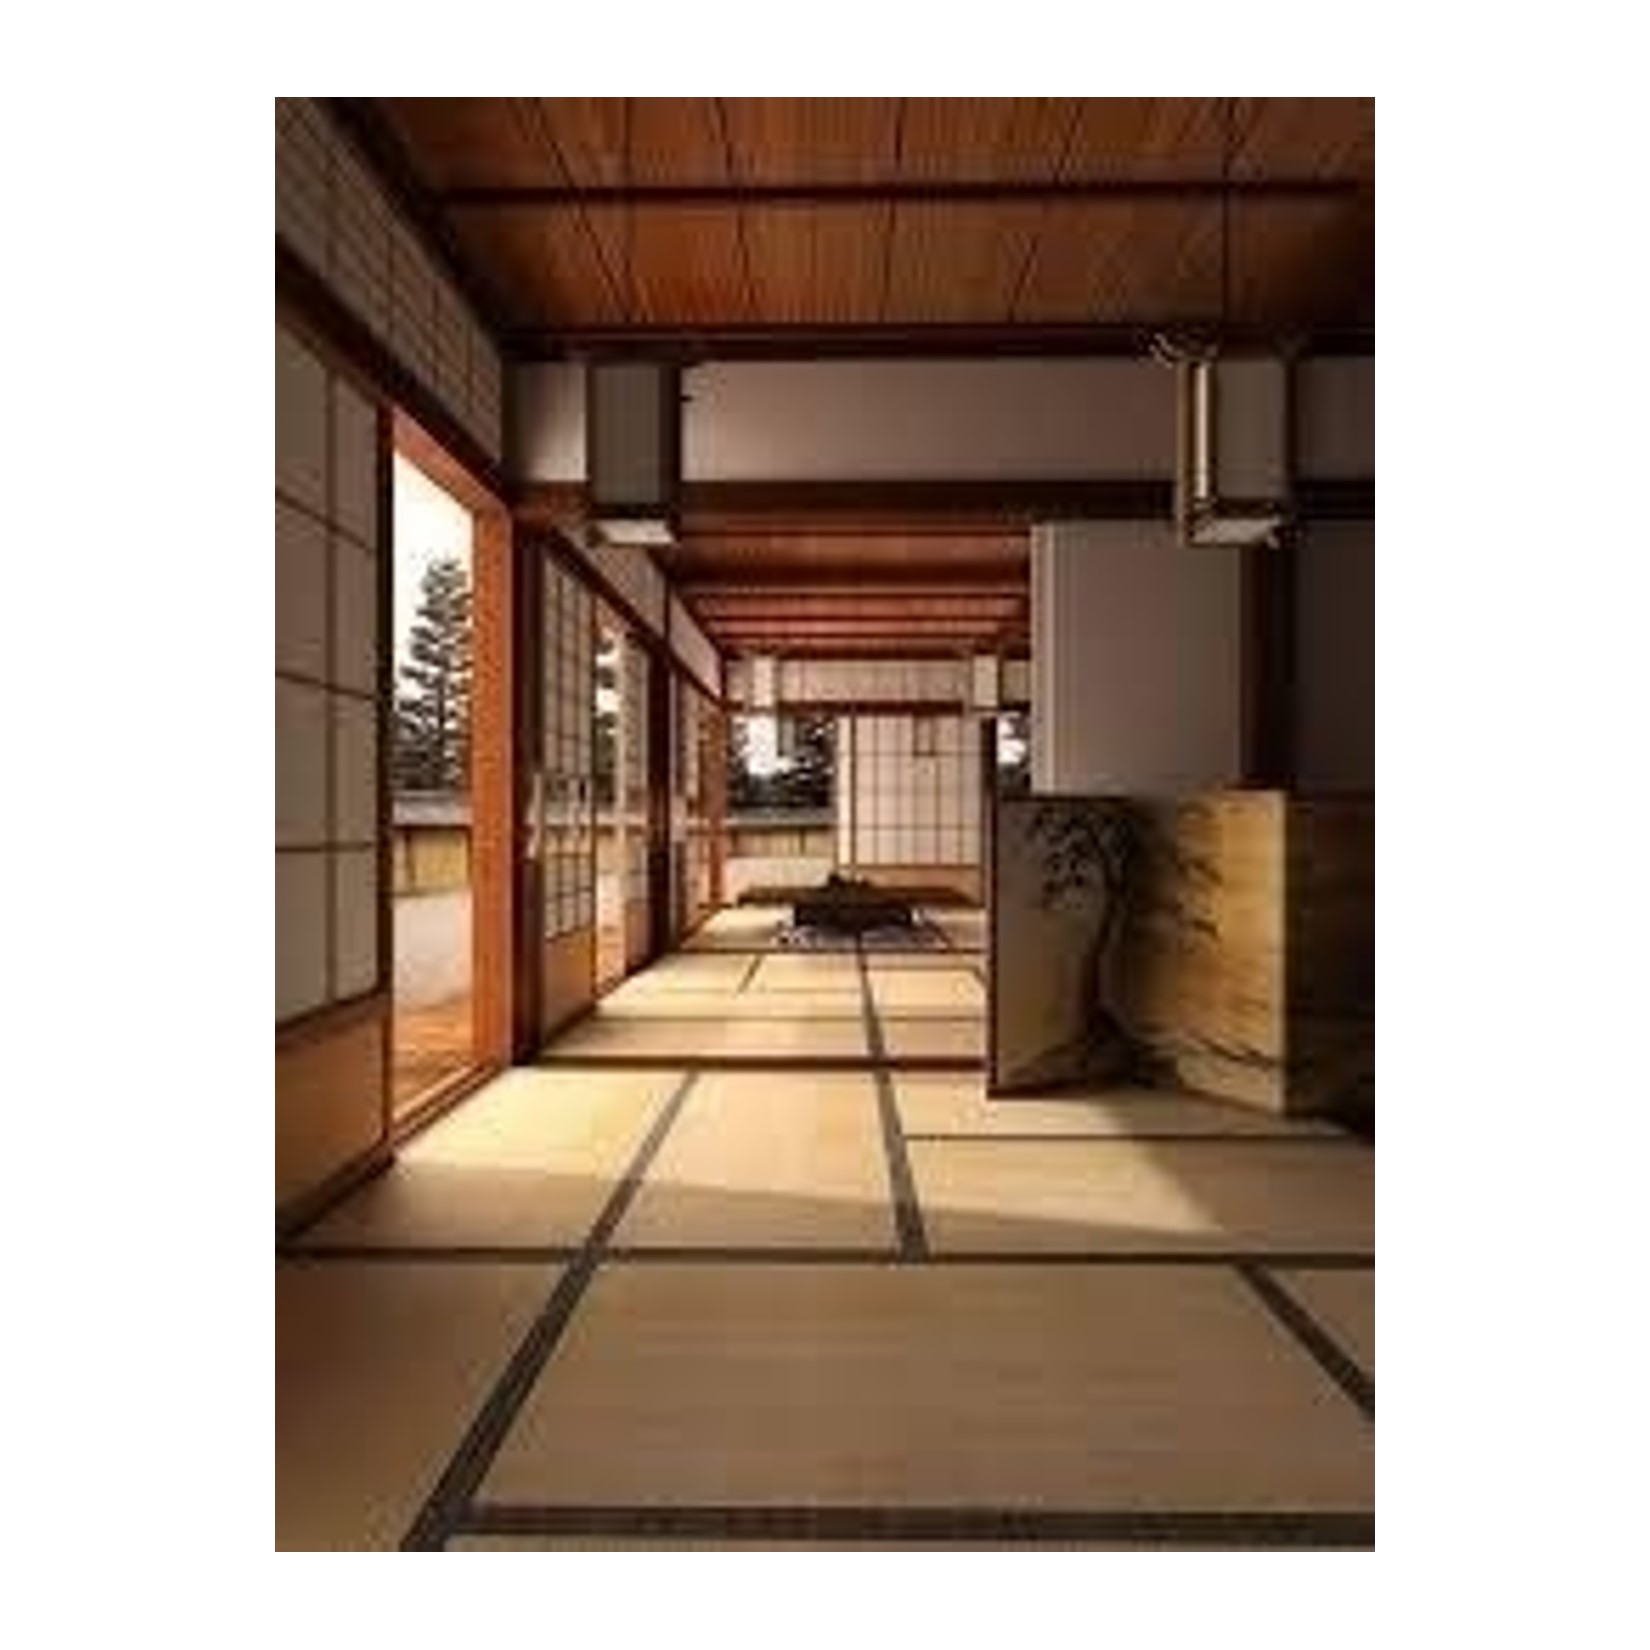
\includegraphics[width=\columnwidth]{CJA.jpg}
\caption{Japanese - Absent.}
\end{subfigure}
\begin{subfigure}[b]{0.3\columnwidth}
\centering

\includegraphics[width=\columnwidth]{CSA.jpg}
\caption{Scandinavian - Absent.}
\end{subfigure}
\caption{Samples from the CARPET dataset.}
\label{ch2:fig:casestudy:2}
\end{figure*}
%

\section{Dataset Analysis}
\label{ch2:sec:dataset_analysis}
To rigorously evaluate the underlying characteristics of the curated datasets, a quantitative analysis framework based on deep feature characterization was implemented. This methodology facilitates an objective assessment of class separability, inter-class overlap, and cluster compactness within a high-dimensional manifold, aligning with established paradigms in visual representation learning \citep{bengio2013representation}.

The computational pipeline was established using the TensorFlow ecosystem \citep{abadi2016tensorflow}. 
A fundamental challenge in image dataset analysis involves the transition from high-dimensional raw pixel intensities to meaningful semantic representations. 
To bridge this gap, we employed the ResNet50 architecture \citep{He_2016_CVPR}, pre-trained on the ImageNet corpus, to serve as a fixed feature extractor.

To accommodate domain-specific visual scales, images within the LAMP dataset were rescaled to $120 \times 120$ pixels, whereas the CARPET dataset utilized a $200 \times 200$ pixel resolution. By removing the terminal fully connected layer and applying Global Average Pooling (GAP), each image $x_i \in \mathcal{X}$ is projected onto a latent feature vector $z \in \mathbb{R}^{2048}$. This dimensionality ensures that the extracted embeddings encapsulate the complex morphological and textural nuances inherent to the specific domain geometries. To prevent subsequent distance metrics from being influenced by varying feature magnitudes, the embedding space is normalized via Z-score standardization using the Scikit-learn library \citep{pedregosa2011scikit}. 

To quantitatively evaluate the internal structure of the defined clusters, we utilize metrics that characterize the distribution of the latent embeddings. Let $k \in \mathcal{K}$ represent a specific data cluster, and let $Z_k = \{z_{1}, z_{2}, \dots, z_{n_k}\}$ be the set of $n_k$ feature vectors belonging to that cluster.The centroid of each cluster, $\mu_k$, is defined as the mean vector of its constituent embeddings:$$\mu_k = \frac{1}{n_k} \sum_{z \in Z_k} z$$

To measure the dispersion of data within a single cluster, we calculate the Mean Intra-cluster Distance ($D_{intra}$), which represents the average Euclidean distance between each point and its respective centroid:$$D_{intra}(k) = \frac{1}{n_k} \sum_{z \in Z_k} \|z - \mu_k\|_2$$A lower value of $D_{intra}$ signifies higher cluster compactness, suggesting that the visual features of the objects within that specific culture or class are highly consistent.

To assess the distinction between different clusters (e.g., between "Lamp On" and "Lamp Off" across different cultures), we employ the Inter-cluster Centroid Distance:$$D_{inter}(k_i, k_j) = \|\mu_{k_i} - \mu_{k_j}\|_2$$In the context of culturally competent ML, a high $D_{inter}$ between the same class across different cultures (e.g., $k_i = (\text{on, Chinese})$ and $k_j = (\text{on, French})$) indicates significant visual variance, which confirms the necessity of culture-aware modeling.

Finally, to provide a holistic view of the dataset's separability, we compute the Silhouette Coefficient $s(i)$ for each sample $z_i$, which balances intra-cluster cohesion and inter-cluster separation:$$s(i) = \frac{b(i) - a(i)}{\max\{a(i), b(i)\}}$$where $a(i)$ is the average distance to other samples in the same cluster and $b(i)$ is the average distance to samples in the nearest neighboring cluster. 
The mean Silhouette score for the entire dataset serves as a proxy for the overall difficulty of the classification task within the latent manifold.

\section{Dataset Analysis Metrics}
\label{ch2:sec:metrics}
This section delineates the mathematical metrics employed to quantify the structural properties and feature distributions of the curated datasets.
To evaluate the internal consistency of each cluster $k \in \mathcal{K}$, we utilize the Mean Intra-Cluster Distance. 
For a cluster containing $n$ samples, the metric is defined as the arithmetic mean of the Euclidean distances between all unique pairs of feature vectors within that cluster:$$ d_{intra}(k) = \frac{2}{n(n-1)} \sum_{i=1}^{n} \sum_{j=i+1}^{n} \| z_i - z_j \|_2 $$where $z_i, z_j \in Z_k$ represent latent feature embeddings belonging to the same cluster. This metric serves as a robust proxy for cluster variance; lower values signify a highly homogeneous category characterized by minimal internal noise and consistent morphological features. 
Conversely, elevated values suggest significant visual diversity within the cultural or class-based grouping.

To quantify the separation between distinct data partitions, we first compute the global centroid $\mu_{k}$ for each cluster $k \in \mathcal{K}$. 
The Inter-Cluster Distance is subsequently defined as the Euclidean distance between the centroids of a cluster pair $(k_i, k_j)$:$$ d_{inter}(k_i, k_j) = \| \mu_{k_i} - \mu_{k_j} \|_2 $$
This metric facilitates the identification of potential "proximity zones" or regions of high similarity in the feature space, where different classes or cultural groupings may converge. 
In the context of classification, lower values of $d_{inter}$ indicate a higher probability of inter-class confusion, suggesting that the model may struggle to differentiate between categories due to overlapping latent representations

%Separation Ratio ($R$) is defined as $\bar{d}_{inter} / \bar{d}_{intra}$, providing a singular heuristic for the overall ``spread'' of the data.

The Silhouette Coefficient ($s$) is a validation metric introduced by Rousseeuw \citep{rousseeuw1987silhouettes} to quantify the degree of similarity between a sample and its assigned cluster relative to other clusters. For a given sample $i$, the coefficient is defined as:$$ s(i) = \frac{b(i) - a(i)}{\max\{a(i), b(i)\}} $$where $a(i)$ represents the mean distance to all other samples within the same cluster, and $b(i)$ denotes the mean distance to samples in the nearest neighboring cluster. 
In accordance with established literature \citep{9260048}, the magnitude of the Silhouette score is interpreted as follows:$s(i) \approx +1$: Indicates that the data point is optimally clustered, exhibiting high cohesion with its assigned group and significant separation from alternative clusters.
$s(i) \approx 0$: Suggests that the data point is situated near the decision boundary between two clusters, indicating potential overlap or ambiguous membership.
$s(i) \approx -1$: Implies that the data point has likely been misclassified or assigned to an incorrect cluster, as it is closer to a neighboring cluster than to its own.

%
\begin{table}[ht]
\centering
\caption{Specific Intra-class Distances for Carpet Sub-categories.}
\label{ch2:tab:carpet_intra}
\begin{tabular}{@{}lcc@{}}
\toprule
\textbf{Config.} & \textbf{Intra-class Distance} "With" &  \textbf{Intra-class Distance} "Without" \\
 \midrule
Binary & 65.12 &  60.12 \\ 
\midrule
 Culture: Indian & 66.82 & 60.99 \\
 Culture: Japanese & 67.29 & 57.61 \\
 Culture: Scandinavian & 56.42 & 57.31 \\ 
\bottomrule
\end{tabular}
\end{table}
%
%
\begin{table}[ht]
    \centering
    \caption{Global Metrics and Intra-class Distances for Carpet Dataset.}
    \label{ch2:tab:carpet_results}
    \begin{tabular}{@{}lcc@{}}
    \toprule
    \textbf{Metric} & \textbf{Binary} & \textbf{Cultural Distinctions} \\ 
    \midrule
    Mean Intra-class Distance & 62.62 & 61.07 \\
    Mean Inter-class Distance & 10.79 & 16.79 \\
    %Separation Ratio ($R$) & 0.1723 & 0.2749 \\
    Silhouette Score ($s$) & 0.0140 & -0.0103 \\ 
    \bottomrule
    \end{tabular}
\end{table}

\begin{table}[ht]
\centering
\caption{Global Metrics and Intra-class Distances for Lamp Dataset.}
\label{ch2:tab:lamp_results}
\begin{tabular}{@{}lcc@{}}
\toprule
\textbf{Metric} & \textbf{Binary} & \textbf{Cultural Distinctions} \\
\midrule
Mean Intra-class Distance & 62.05 & 59.35 \\
Mean Inter-class Distance & 6.19 & 18.38 \\
%Separation Ratio ($R$) & 0.0997 & 0.3097 \\
Silhouette Score ($s$) & 0.0052 & -0.0367 \\ 
\bottomrule
\end{tabular}
\end{table}

\begin{table}[ht]
\centering
\caption{Specific Intra-class Distances for Lamp Sub-categories.}
\label{ch2:tab:lamp_intra}
\begin{tabular}{@{}llc@{}}
\toprule
\textbf{Config.} & \textbf{Binary} & \textbf{Cultural Distinctions} \\
\midrule
Binary & \textbf{Intra-class Distance} "Off" &  \textbf{Intra-class Distance} "On" \\ 
\midrule
Culture Chinese &  70.20 & 67.42 \\
Culture French & 48.21 & 53.86 \\
Culture Turkish & 60.99 & 55.42 \\ 
 \bottomrule
\end{tabular}
\end{table}

%The Lamp dataset benefits more significantly from multiclass labeling, showing a sharper increase in the Separation Ratio than the Carpet dataset. 
%However, 
The CARPET dataset exhibits a marginally higher Silhouette score, suggesting that textile textures possess a more stable distribution within the ResNet50 manifold relative to the more volatile geometric features of the LAMP objects. In both instances, the observed relationship $\bar{d}_{intra} \gg \bar{d}_{inter}$ indicates that these datasets are characterized by high-variance distributions. Such structural properties suggest that linear separation may be insufficient, potentially necessitating non-linear classification strategies or domain-specific fine-tuning to achieve robust predictive performance.

\begin{figure}
    \centering
    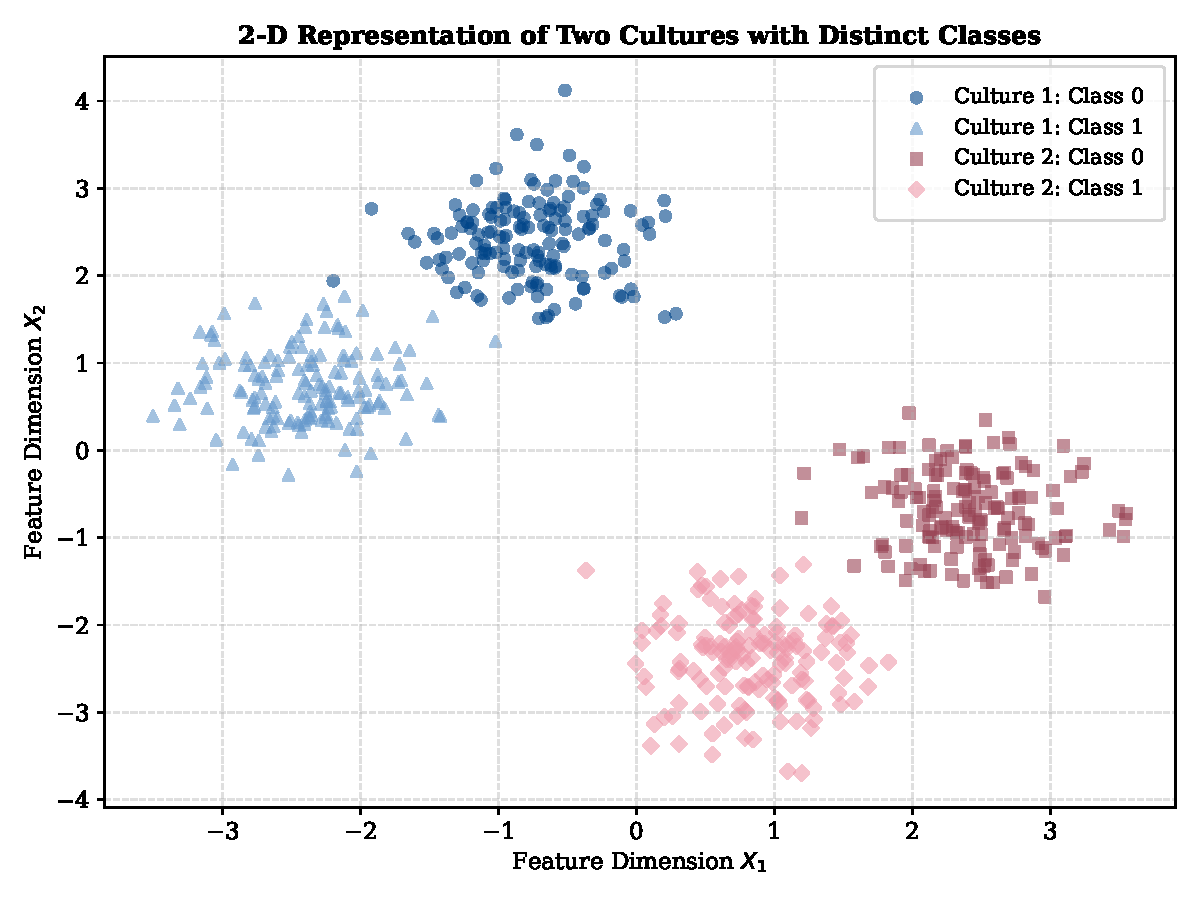
\includegraphics[width=1.0\linewidth]{Chapter2/Figs/2-DRepresentationOfDatasetDistributions.pdf}
    \caption{2-D Representation of intra and extra classes analysis of the LAMP or CARPET datasets.}
    \label{ch2:fig:2dDatasetDistribution}
\end{figure}

This analysis validates an intuitive understanding of the latent feature space: the visual variance introduced by a state transition (e.g., a lamp being in an "active" versus "inactive" state) is significantly lower than the structural variance inherent between distinct object categories. 
Specifically, the latent representation of a Japanese-style domestic interior remains highly consistent regardless of the presence of a carpet, whereas heterogeneous lamp models introduce substantial geometric shifts. 
This phenomenon explains why the intra-class distances within the binary, state-based classification paradigm consistently exceed the inter-class distances, resulting in the significant cluster overlap observed in our quantitative metrics.

A simplified two-dimensional projection of the intra-class and inter-class distribution analysis is illustrated in Figure~\ref{ch2:fig:2dDatasetDistribution}.

\section{ML Preliminaries}
\label{ch2:sec:prel}
In a classical ML framework~\citep{shalev2014understanding,goodfellow2016deep,aggarwal2023neural}, a dataset $\mathcal{D}_n = \{ (x_1, y_1), \dots, (x_n, y_n) \}$ is utilized, consisting of $n$ samples drawn independently and identically distributed (i.i.d.) from an unknown joint probability distribution $\mu$ over the product space $\mathcal{X} \times \mathcal{Y}$. 
Here, $\mathcal{X}$ represents the high-dimensional input space (e.g., feature vectors or raw pixel data), and $\mathcal{Y}$ denotes the corresponding label or output space.

Within this setting, the objective is to derive a predictive model $f_\Theta: \mathcal{X} \rightarrow \mathcal{Y}$, parameterized by $\Theta$, by means of a learning algorithm $\mathscr{A}_\mathcal{H}$ governed by a set of hyperparameters $\mathcal{H}$. The algorithm selects the optimal hypothesis $f_\Theta$ from the hypothesis space based on the evidence provided by $\mathcal{D}_n$, with the aim of accurately approximating the posterior distribution $\mathbb{P}(Y|X)$.
The fidelity of this approximation is quantified through a loss function $\ell: \mathcal{Y} \times \mathcal{Y} \rightarrow \mathbb{R}$, which measures the discrepancy between predicted and ground-truth values. For example, if $\mathcal{Y} = \{-1, +1\}$, the task is formulated as a binary classification problem; conversely, if $\mathcal{Y} \subset \mathbb{R}$, the task is defined as a regression problem.

The set of hyperparameters $\mathcal{H}$ encompasses several critical architectural and algorithmic factors~\citep{shalev2014understanding,goodfellow2016deep,aggarwal2023neural}. These include the functional form of $f_\Theta$ (e.g., linear models, kernel methods, or deep architectures such as convolutions and transformers), the specific parameterization of said form (e.g., kernel selection, layer depth, and width), and regularization strategies. 
The latter may include explicit techniques, such as the selection and magnitude of norm-based penalties, or implicit regularization induced by the choice of optimizer, early stopping criteria, and dropout mechanisms.In a generalized form, the model $f_\Theta$ can be represented as a linear combination of features:\begin{align}\label{ch2:eq:function}f(x) = \mathbf{w}^\top \varphi(x)\end{align}where $\varphi(\cdot)$ denotes a mapping (possibly non-linear) from the input space to a feature space, and $\mathbf{w}$ represents the weight vector.
%
When the feature mapping $\varphi: \mathcal{X} \rightarrow \mathbb{R}^d$ is fixed—whether explicitly through manual feature engineering~\citep{duboue2020art}, by leveraging a frozen backbone from a model zoo~\citep{shu2021zoo}, or implicitly via the use of kernels~\citep{shalev2014understanding}—the parameter set is restricted to $\Theta = \mathbf{w} \in \mathbb{R}^d$. 
This configuration constitutes what is formally categorized as a shallow model.
Conversely, when $\varphi$ is itself parameterized by a set of weights $W$—as seen in the filters of a convolutional neural network~\citep{goodfellow2016deep}, the learnable coefficients of an activation function~\citep{apicella2021survey}, or the lower layers of a pre-trained network undergoing fine-tuning~\citep{shu2021zoo}—then $\Theta = \{ \mathbf{w}, W \}$. 
In this scenario, the architecture is classified as a deep model, where the feature representation and the classifier are optimized jointly.
Finally, when $\varphi$ represents the aggregated outputs of a population of weak learners, which may or may not be individually parameterized by $W$ (e.g., decision trees generated via bagging, boosting, or hybrid strategies), and $\mathbf{w}$ denotes either fixed constants or learned integration weights, the approach is defined as an ensemble model~\citep{sagi2018ensemble}.

In the absence of a priori knowledge regarding the underlying distribution $\mu$, the parameter set $\Theta$ and the hyperparameter configuration $\mathcal{H}$ are derived exclusively from the empirical evidence provided by $\mathcal{D}_n$. 
This process occurs during the training and model selection phases, respectively~\citep{shalev2014understanding,oneto2014fully,OnetoB003}.

Typically, the training phase is formulated as the following optimization problem:%
\begin{align}\label{ch2:eq:generalproblem}\min_\Theta \quad \hat{\mathbb{E}}{\mathcal{D}n} \left[ \ell(f\Theta(x), y) \right] + R(\Theta),
\end{align}
%
where $\hat{\mathbb{E}}{\mathcal{D}_n}$ denotes the empirical expectation (or empirical risk) computed over the samples $(x, y) \in \mathcal{D}_n$.
In essence, once the hyperparameter set $\mathcal{H}$ is fixed, a Regularized Empirical Risk Minimization (RERM) procedure is executed. 
Within this framework, certain hyperparameters are explicitly manifested—for instance, as regularization coefficients within the penalty term $R(\Theta)$—whereas others remain implicitly embedded within the architectural constraints of the functional form $f_\Theta$ or the dynamics of the optimization process ($\min$).

Upon the resolution of Problem~\eqref{ch2:eq:generalproblem}, the predictive performance of the learning algorithm $\mathscr{A}_\mathcal{H}$—specifically its capacity to identify an optimal hypothesis $f_\Theta$ that generalizes to unseen data—is optimized during the model selection phase and quantified during the risk estimation phase~\citep{OnetoB003}.In practice, resampling techniques are widely adopted due to their versatility and robustness across diverse data distributions. 
These methods are predicated on a fundamental heuristic: the primary dataset $\mathcal{D}_n$ is partitioned, either through a single instance or multiple iterations ($n_r$), into three mutually exclusive subsets. 
These are designated as the learning ($\mathcal{L}^r$), validation ($\mathcal{V}^r$), and test ($\mathcal{T}^r$) sets, for $r \in \{ 1, \dots, n_r \}$. To ensure the integrity of the evaluation, these subsets are constructed such that:$$ \mathcal{L}^r \cap \mathcal{V}^r = \emptyset, \quad \mathcal{L}^r \cap \mathcal{T}^r = \emptyset, \quad \mathcal{V}^r \cap \mathcal{T}^r = \emptyset $$$$ \mathcal{L}^r \cup \mathcal{V}^r \cup \mathcal{T}^r = \mathcal{D}_n $$Subsequently, to identify the optimal hyperparameter configuration $\mathcal{H}^*$ from a candidate space $\mathcal{S} = \{ \mathcal{H}_1, \mathcal{H}_2, \dots \}$, the model selection phase proceeds according to the following formal procedure.
%
The model selection phase is formally defined as the optimization of the hyperparameter configuration $\mathcal{H}$ over the candidate space $\mathcal{S}$ to minimize the validation risk:\begin{align}\label{ch2:eq:MS}\mathcal{H}^* = \arg\min_{\mathcal{H} \in \mathcal{S}} \quad\hat{\mathbb{E}}r \left[ \hat{\mathbb{E}}{\mathcal{V}^r} \left[ \ell(\mathscr{A}_{\mathcal{H}}(\mathcal{L}^r)(x), y) \right] \right],\end{align}where $\hat{\mathbb{E}}_r$ denotes the empirical expectation over the $n_r$ resampling iterations, and $f_{\Theta^*} = \mathscr{A}_{\mathcal{H}}(\mathcal{L}^r)$ represents the hypothesis generated by the algorithm $\mathscr{A}_\mathcal{H}$—governed by the hyperparameter set $\mathcal{H}$—when trained on the learning set $\mathcal{L}^r$.
Because the samples $(x, y) \in \mathcal{V}^r$ are excluded from the training phase, the validation set serves as an unbiased proxy for the true distribution $\mu$. 
Consequently, the selected optimal hyperparameter configuration $\mathcal{H}^*$ is that which minimizes the empirical risk on this previously unseen data, thereby mitigating the risk of overfitting to the training distribution.
Subsequently, to evaluate the performance of the optimal model—specifically, the model $f_{\Theta^*}$ resulting from the optimization in Problem~\eqref{ch2:eq:generalproblem} utilizing the optimal hyperparameter configuration $\mathcal{H}^*$ derived from Problem~\eqref{ch2:eq:MS}—the Generalization Error (ERR) is computed on the test set:
%
\begin{align}
\label{ch2:eq:EE}
\text{ERR} = \hat{\mathbb{E}}r \left[ \hat{\mathbb{E}}{\mathcal{T}^r} \left[ \ell(\mathscr{A}_{\mathcal{H}^*}(\mathcal{L}^r \cup \mathcal{V}^r)(x), y) \right] \right],
\end{align}
%
where $f_{\Theta^*} = \mathscr{A}_{\mathcal{H}^*}(\mathcal{L}^r \cup \mathcal{V}^r)$ represents the hypothesis generated by the algorithm $\mathscr{A}$ using the optimal hyperparameters $\mathcal{H}^*$ and the combined learning and validation data $\mathcal{L}^r \cup \mathcal{V}^r$.
As the test partitions $\mathcal{T}^r$ are strictly withheld from both the training phase in Eq.~\eqref{ch2:eq:generalproblem} and the model selection phase in Eq.~\eqref{ch2:eq:MS}, ERR serves as an unbiased estimator of the model's generalization capacity. 
Formally, this metric quantifies the fidelity of the approximation of the posterior distribution $\mathbb{P}(Y|X)$ when encountering previously unseen data points~\citep{OnetoB003}.

Counterintuitively, it should be noted that the loss function $\ell$ employed during the training phase may deviate from the metric utilized during the model selection and risk estimation phases. This strategic divergence is often implemented to enhance training effectiveness and computational efficiency~\citep{rosasco2004loss,shalev2014understanding,goodfellow2016deep,aggarwal2023neural}.
Specifically, while the application may require a non-convex or non-differentiable metric—such as the $0/1$ loss for classification—training typically necessitates a surrogate loss function (e.g., Cross-Entropy or Hinge loss) that is convex and differentiable, thereby facilitating the use of gradient-based optimization methods.

\section{Culturally Competent ML}
\label{ch2:sec:makeMLcultcomp}
This section delineates the theoretical framework for developing ML models constrained by principles of cultural competency.
\subsection{Quantifying Cultural Incompetence}
\label{ch2:sec:CCML}
In the context of culturally competent ML, we consider a dataset $\mathcal{D}_n = \{ (x_1, c_1, y_1), \dots, (x_n, c_n, y_n) \}$. 
Diverging from the classical ML paradigm, each sample is augmented with a reference cultural context $c \in \mathcal{C}$, where $\mathcal{C}$ represents a set of discrete cultural identifiers (e.g., Chinese, French, Turkish, Indian, Japanese, and Scandinavian).It is important to acknowledge the simplifying assumption that cultural contexts are distinct, well-defined, and enumerable. 
While this taxonomical approach is computationally advantageous for labeling data collected across disparate geographic regions, it represents an abstraction of reality. 
As discussed in Section~\ref{ch1:sec:introduction}, culture is inherently fluid and non-discrete. 
For instance, interior design paradigms and gastronomic preferences within a single nationality, such as the Italian population, exhibit significant non-homogeneity. 
Such variations are driven by regional ontologies, personal trajectories, familial traditions, and individual predispositions—latent variables that are not explicitly captured within the categorical space $\mathcal{C}$

In this study, we assume the availability of the cultural context $c$ for all observations, such that $c$ is known $\forall (x, c, y) \in \mathcal{D}_n$. 
While this constitutes a significant assumption, it is a constraint that can be relaxed in more complex scenarios, as demonstrated in the literature on algorithmic fairness~\citep{survey_fairness_wreprbias,oneto2019taking}.
In a practical deployment, $c$ may be observable only for a sparse subset of $\mathcal{D}_n$ or entirely latent. 
Furthermore, it might be available exclusively during the model construction phase (training and model selection) but unavailable during the inference (forward) phase. 
Notwithstanding these potential complexities, the present work adheres to a foundational framework where $c$ is assumed to be fully observable across the entirety of $\mathcal{D}_n$.

Based on these premises, culturally competent ML transcends the singular objective of approximating $\mathbb{P}(Y|X)$ via a standard loss function $\ell$. Instead, it incorporates a secondary objective: the minimization of performance disparity across diverse cultural contexts. 
Formally, the goal is to achieve an accurate approximation of the conditional probability $\mathbb{P}(Y|X, C)$ for every cultural context $c \in \mathcal{C}$.
In practice, the dataset $\mathcal{D}_n$ may exhibit representational bias~\citep{not_uniform_data}, wherein $\mathbb{P}(Y|X, C)$ is under-represented for specific cultural identifiers $c \in \mathcal{C}$—either due to a lower cardinality of samples or the presence of degraded signal quality within those subsets. 

Furthermore, classical ML algorithms optimized solely for $\mathbb{P}(Y|X)$ tend to favor "shortcuts" to optimize global performance~\citep{geirhos2020shortcut,cristianini2023shortcut}. 
By failing to explicitly account for the requirement to accurately model $\mathbb{P}(Y|X, C)$ $\forall c \in \mathcal{C}$, these models often achieve high aggregate accuracy at the expense of significant, and often systematic, performance degradation within minority or under-represented cultural strata.
%For example, for the CARPET dataset, which is one of the datasets described in Section~\ref{ch2:sec:data}, the model could leverage some background properties, instead of focusing on the floor, that is, of course, different depending on the culture to over-perform in some culture with respect to another one.
For instance, within the CARPET dataset detailed in Section~\ref{ch2:sec:data}, a model may exhibit a propensity for "shortcut learning" by relying on auxiliary background characteristics rather than the salient features of the floor itself. 
This is particularly problematic given the significant variance in domestic background environments across disparate cultural contexts. 
Such a dependency induces a systematic bias, causing the model's predictive performance to fluctuate significantly when evaluated across different cultural strata.
To mitigate these representational discrepancies, the present work focuses on the development of models capable of the simultaneous optimization of the following metrics $\forall c \in \mathcal{C}$:
%
\begin{align}
\label{ch2:eq:EEC}
\text{ERR}^C = \hat{\mathbb{E}}_r
\hat{\mathbb{E}}_{ \mathcal{T}^{r,C}} \ell(\mathscr{A}_{\mathcal{H}^*}(\mathcal{L}^r {\cup} \mathcal{V}^r)(X),Y),
\end{align}
%
where $\mathcal{T}^{r,c} = \{ (x, c', y) : c' = c, (x, c', y) \in \mathcal{T}^r \}$ $\forall c \in \mathcal{C}$.
The term $\text{ERR}^c$ represents the cultural generalization error (analogous to the global $\text{ERR}$ defined in Eq.~\ref{ch2:eq:EE}). 
This metric is derived by evaluating the optimal model—previously trained and validated on the aggregate dataset—exclusively on the subset of test samples associated with the specific cultural context $c$. 
It should be noted that $\text{ERR}^c$ constitutes an unbiased estimator of the model's generalization capacity for each discrete culture; specifically, it quantifies the fidelity of the approximation of the conditional probability $\mathbb{P}(Y|X, C)$ within that specific cultural stratum.

We then define the measure of Cultural Incompetence (CIC) as follows:
%
\begin{align}\label{ch2:eq:cic}
\text{CIC} = \hat{\mathbb{E}}c \left[ \left| \text{ERR}^c - \min{c' \in \mathcal{C}} \text{ERR}^{c'} \right| \right],
\end{align}
%
where $\hat{\mathbb{E}}_c = \frac{1}{|\mathcal{C}|} \sum_{c \in \mathcal{C}}$ denotes the empirical expectation over the set of cultural contexts $\mathcal{C}$.
he underlying principle is that, upon identifying the reference cultural context $c'$ for which the error $\text{ERR}^{c'}$ is minimized, the objective is to ensure that all other cultural contexts $c \in \mathcal{C}$ exhibit comparable predictive performance. Essentially, the goal is to minimize the performance gap relative to this best-case baseline.Consider the previously mentioned scenario involving the cross-border commercialization of a SR. 
A high CIC value indicates a lack of cultural robustness: while the robot may accurately perceive its physical and social environment within its native cultural context $c'$ (characterized by a low $\text{ERR}^{c'}$), its performance degrades significantly when deployed in alternative cultural settings (where $\text{ERR}^c \gg \text{ERR}^{c'}$ for $c \neq c'$).
To rigorously assess a robot's readiness for multi-contextual deployment, the CIC should be re-evaluated for each specific task the agent must execute, encompassing the full spectrum of relevant cultural identifiers. 
In the subsequent sections of this work, we utilize the CIC metric to quantify the efficacy of our proposed framework in enhancing algorithmic cultural competency. 
This enables a formal comparison between our methodology and traditional, culturally agnostic approaches.

Given our formalized definition of cultural competency, our primary objective is to isolate and quantify the discrepancy in performance across cultural contexts, independent of the relative proportions or frequencies with which these cultures are represented in the training distribution. This discrepancy is mathematically expressed as the mean deviation between the performance achieved in the most proficiently modeled culture and the performance across all remaining cultural strata.Within this framework, we adopt $\min_{c' \in \mathcal{C}} \text{ERR}^{c'}$ as the benchmark for optimal performance. This selection is necessitated by the fact that global model accuracy (the absolute error rate) and cultural competency (the relative error variance) are distinct properties; a model may exhibit suboptimal aggregate performance on a given task while simultaneously demonstrating high cultural competency by maintaining consistent error rates across all cultural identifiers.

It is important to clarify that the notation $\text{ERR}$ may inadvertently imply a generic average error. 
However, as formalized in Equations~\eqref{ch2:eq:EE} and \eqref{ch2:eq:EEC}, $\text{ERR}$ represents an estimation of the expected risk, the interpretation of which is contingent upon the specific loss function $\ell$ dictated by the problem domain. 
Consequently, the terms $\text{ERR}$, $\text{ERR}^c$, and $\text{CIC}$ are utilized as generalized metrics throughout this discourse.
Furthermore, the $\text{CIC}$ metric alone is insufficient to characterize a model as culturally competent. 
A low $\text{CIC}$ value merely indicates parity across cultural contexts; if the aggregate $\text{ERR}$ is excessively high, the model remains functionally incompetent across all cultures despite the lack of disparity. 
In such a state, the $\text{ERR}^c$ values would be uniformly poor, yielding a low $\text{CIC}$ that masks a failure in basic predictive utility.
Therefore, the ultimate objective of a culturally competent framework is the simultaneous minimization of both the global risk ($\text{ERR}$) and the cultural incompetence ($\text{CIC}$). 
A schematic representation of the classical ML pipeline is provided in Figure~\ref{ch2:fig:MLflow} for comparison.

%
\begin{figure*}
    \centering
    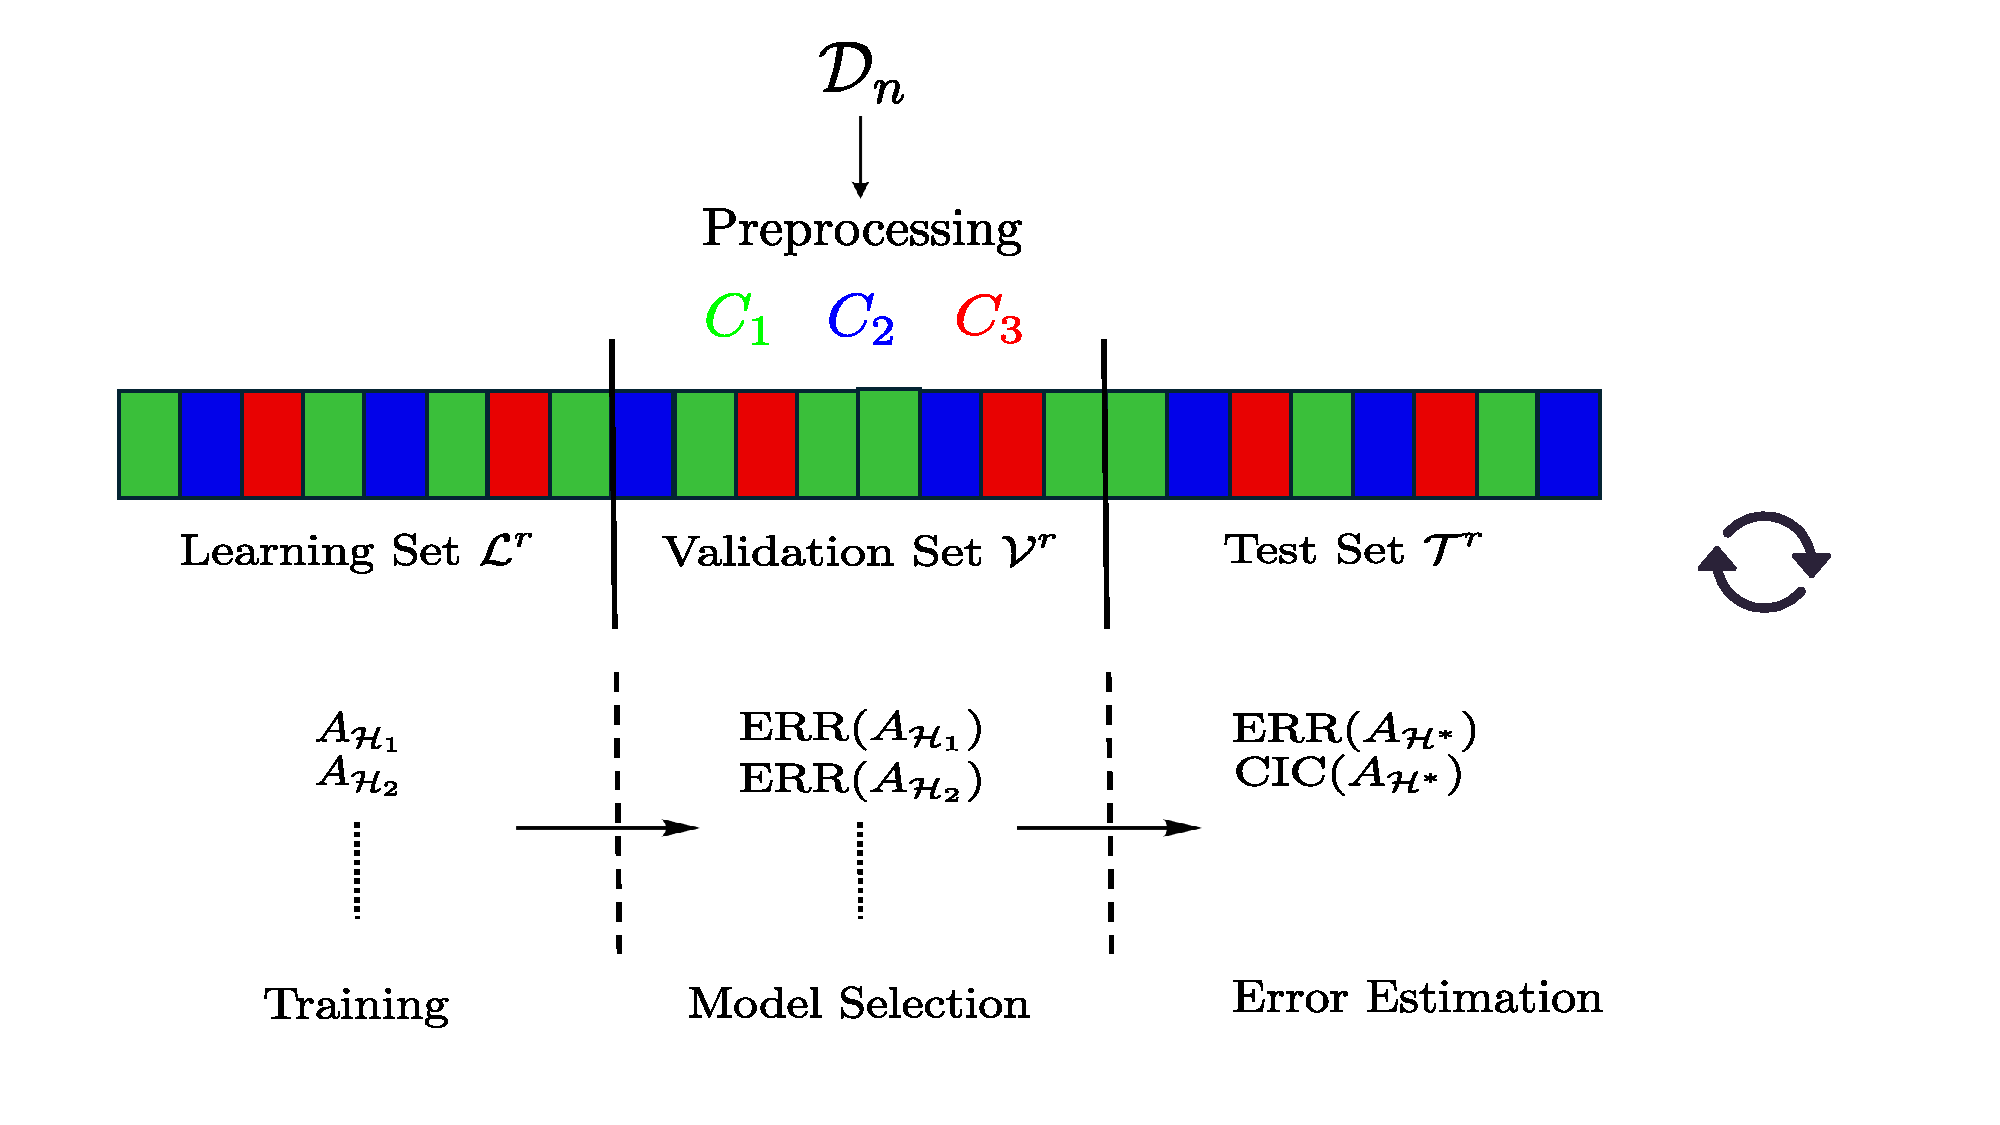
\includegraphics[width=\linewidth]{MLFlowchart.pdf}
    \caption{Classical ML framework and CIC measurement.}
    \label{ch2:fig:MLflow}
\end{figure*}

\section{Multi-Task-Learning-Inspired Mitigation Strategy}
\label{ch2:sec:mtl}

This section delineates our primary methodology for embedding cultural competency within ML models, inspired by the MTL paradigm.

It should be noted that the proposed approach was evaluated using the ResNet architecture to facilitate a rigorous performance comparison with its culturally agnostic baseline. The selection of ResNet was motivated by its superior performance on the LAMP dataset when evaluated through traditional metrics. 
However, the methodology remains fundamentally architecture-agnostic and may be generalized or adapted to a wide array of ML frameworks.

The proposed framework is predicated on addressing the primary factors contributing to cultural incompetence.

The foremost challenge involves the representational disparity of cultural groups within the training distribution. 
This phenomenon may arise from several systemic factors. Primarily, certain cultures may be under-represented due to inherent imbalances in data collection—resulting in either a lower sample cardinality or a diminished signal-to-noise ratio (e.g., degraded data quality or inconsistent labeling)—for specific cultural identifiers.
%The second reason is that a model has been first developed in a country collecting data in that specific country, therefore reflecting just one culture.
A secondary challenge arises from the geographical and cultural centering of initial model development. 
Specifically, a system may be prototyped and trained within a singular cultural context, thereby capturing and reflecting the idiosyncratic priors of that specific region.

As the resulting application achieves commercial or functional viability and is subsequently exported to disparate cultural contexts, practical constraints often impede the data acquisition process. 
In these deployment phases, limitations in temporal and financial resources frequently preclude the collection of a longitudinal dataset that matches the cardinality and fidelity of the original developmental corpus. 
Consequently, the model is forced to generalize to novel cultural strata using significantly sparser information.

The second fundamental challenge underlying cultural (in)competence is the dual nature of cultural data, which is characterized by both cross-cultural commonalities and region-specific idiosyncrasies.

Disregarding these cultural nuances—for instance, by deploying a model trained in one cultural context directly into another—yields suboptimal performance, as demonstrated in Section~\ref{ch3}. 
Conversely, and perhaps counterintuitively, developing independent, culture-specific models is also a suboptimal strategy. 
Such a fragmented approach fails to leverage shared structural patterns and information-rich commonalities inherent across disparate cultural datasets, thereby neglecting valuable global features (see Section~\ref{ch3}).

To mitigate these challenges, we propose the integration of a novel, generalized regularization framework within the ML model, drawing inspiration from the MTL paradigm~\citep{zhang2018overview}. 
This regularizer is mathematically formulated to simultaneously compensate for the representational scarcity of certain cultures and exploit cross-cultural commonalities, while maintaining sufficient flexibility to capture unique, context-specific variations.

\begin{figure}
    \centering
    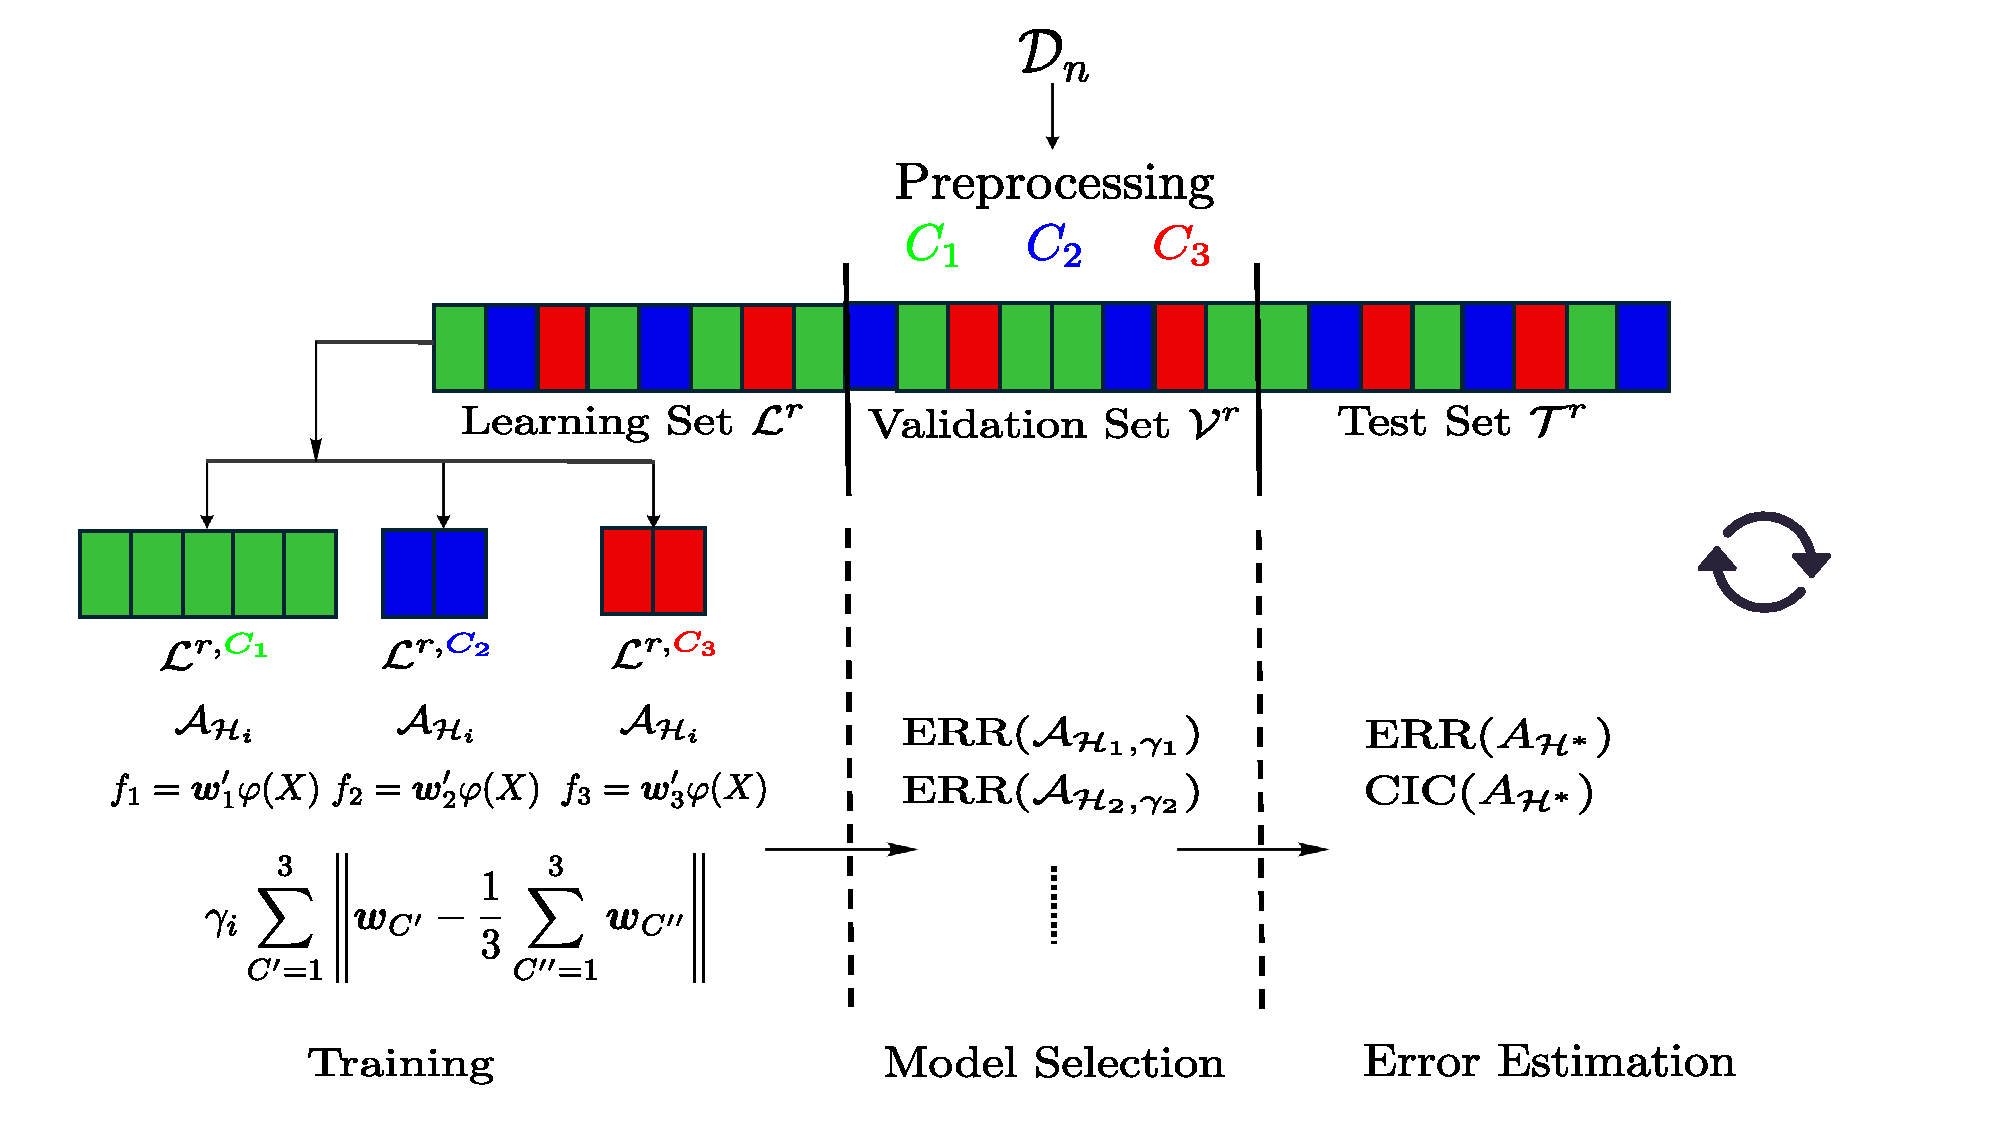
\includegraphics[width=1.2\linewidth]{CCMLFlowchart.pdf}
    \caption{Culturally Competent Multi-task-learning-inspired Mitigation Strategy.}
    \label{ch2:fig:CCMLflow}
\end{figure}

Formally, the mathematical intuition underlying our methodology is as follows: To ensure the model remains sensitive to the unique idiosyncrasies of each cultural context, we instantiate a specific hypothesis for each culture $c \in \mathcal{C}$.
%
\begin{align}
f_{\Theta^C}(X) = \boldsymbol{w}_C \varphi(X), \quad \forall C \in \mathcal{C},
\end{align}
%
Consequently, the classical ML optimization objective defined in Eq.~\eqref{ch2:eq:generalproblem} is reformulated as follows:
%
\begin{align}\label{ch2:eq:generalproblem_mitigation}\min_{\Theta^c, c \in \mathcal{C}}\hat{\mathbb{E}}{c} \left[ \hat{\mathbb{E}}{\mathcal{D}^c_n} \ell(f_{\Theta^c}(x), y) \right] + \sum_{c \in \mathcal{C}} R(\Theta^c),\end{align}
%
where $\mathcal{D}^{c'}_n = \{ (x, c, y) : c = c', (x, c, y) \in \mathcal{D}_n \}$ $\forall c' \in \mathcal{C}$ denotes the cultural partition of the dataset. 
Within this formulation, Problem~\eqref{ch2:eq:generalproblem_mitigation} entails utilizing the same learning algorithm to instantiate a distinct model configuration for each cultural identifier.For instance, in the context of the LAMP dataset utilizing a Linear Support Vector Machine (LSVM), this approach results in the construction of an independent binary classifier for lamp state recognition tailored to each specific cultural context.

This independent formulation remains insufficient. 
By partitioning the dataset into isolated cultural subsets, we fail to exploit the shared structural patterns present across the aggregate data. Consequently, for cultural contexts characterized by limited sample cardinality or degraded signal quality, the model cannot leverage informative commonalities from other cultures that would otherwise enhance its predictive robustness.

To address this limitation, we introduce a regularization term—drawing inspiration from the MTL framework~\citep{zhang2018overview}—to be integrated into the objective function in Problem~\eqref{ch2:eq:generalproblem_mitigation}. This regularizer is specifically designed to facilitate information sharing across cultural boundaries, thereby utilizing universal commonalities to bolster the performance of the model in every cultural stratum.
Specifically, the proposed regularization term assumes the following functional form:
%
\begin{align}
\label{ch2:eq:proposedregularizer}
\gamma \sum_{c \in \mathcal{C}} \left| \boldsymbol{w}{c} - \frac{1}{|\mathcal{C}|} \sum{c' \in \mathcal{C}} \boldsymbol{w}_{c'} \right|_2^2,
\end{align}
%
where $\gamma \in \mathbb{R}^+$ denotes a hyperparameter governing the regularization intensity.
Intuitively, this regularization term incentivizes each culture-specific model $\boldsymbol{w}_{c}$ to remain in proximity to the global cultural centroid, defined as the empirical mean $\frac{1}{|\mathcal{C}|} \sum_{c' \in \mathcal{C}} \boldsymbol{w}_{c'}$. 
This mechanism explicitly models cross-cultural commonalities. 
In the functional form $f(x) = \boldsymbol{w}_c^\top \varphi_c(x)$ (cf. Eq.~\eqref{ch2:eq:function}), the feature extractor $\varphi_c$—which is typically uniform across all cultures—is responsible for mapping the input image into a latent representation space, while the vector $\boldsymbol{w}_c$ defines the culture-specific decision boundary. 
By enforcing a shared $\varphi$ across all cultural contexts, the framework ensures the acquisition of a robust, task-invariant representation. 
Consistent with established transfer learning practices~\citep{shu2021zoo}, a pre-trained backbone is often utilized as the feature extractor, as it provides a foundational representation capable of capturing the diverse nuances inherent in cross-cultural data.
Consequently, the application of the regularizer~\eqref{ch2:eq:proposedregularizer} to the parameters $\boldsymbol{w}_{c}$ enables the model to simultaneously account for cultural idiosyncrasies and exploit shared global features. This dual optimization effectively mitigates the risks associated with data scarcity or degraded signal quality in specific cultural strata by facilitating information transfer from more densely sampled cultural groups.

It should be observed that the functional form of the regularizer~\eqref{ch2:eq:proposedregularizer} exhibits a strong structural parallel to the definition of CIC in Eq.~\eqref{ch2:eq:cic}. This correspondence is deliberate, as CIC effectively represents the application of regularizer~\eqref{ch2:eq:proposedregularizer} to the model outputs rather than the model parameters $\boldsymbol{w}_{c}$.
Drawing from the theoretical foundations of Multi-Task Learning~\citep{zhang2018overview}, it is established that imposing constraints exclusively on the hypothesis outputs is significantly less efficacious than regularizing the hypothesis parameters themselves. 
This disparity in effectiveness arises because the parameter space $\Theta$ encapsulates the structural information and inductive biases of the model, whereas raw outputs provide only a low-dimensional projection of the learned representation.

In summary, our proposed framework for culturally competent ML adopts the optimization objective delineated in Problem~\eqref{ch2:eq:generalproblem_mitigation}, integrating the regularization term defined in Eq.~\eqref{ch2:eq:proposedregularizer}. 
This methodology enables the training of distinct, culture-specific hypotheses while simultaneously enforcing a structural constraint that facilitates information transfer across cultural boundaries.
It is noteworthy that the computational overhead of this approach remains asymptotically comparable to that of training either a monolithic model on the aggregate dataset or independent models for each cultural partition. 
The primary additional requirement involves the optimization of the regularization hyperparameter $\gamma$, the search space for which is detailed in Table~\ref{ch3:tab:hyper}.
%
\subsection{Tuning \texorpdfstring{$\gamma$}{gamma}}
\label{ch2:sec:tuning_gamma}
%
The hyperparameter $\gamma$ performs a critical function by implicitly embedding the CIC metric directly into the learning objective. 
Consequently, the optimization of $\gamma$ cannot be predicated exclusively on the minimization of the expected risk ($\text{ERR}$) within the validation set. 
Instead, the selection process must be driven by a multi-objective criterion that simultaneously accounts for the model's $\text{CIC}$ on the validation data.

This optimization challenge is non-trivial, as the simultaneous minimization of multiple metrics typically yields a set of non-dominated solutions constituting a Pareto frontier~\citep{ishizaka2013multi}. 
To navigate this trade-off, we adopt a bi-level selection strategy inspired by the methodology proposed in~\citep{OnetoC060}.
In the initial stage, we determine the optimal hyperparameter value $\gamma^*$ that minimizes the expected risk ($\text{ERR}$). In the subsequent stage, we define a candidate set of $\gamma$ values that maintain an accuracy threshold within a factor of $(1-\tau)$ of the optimal performance. 
Formally, we shortlist all $\gamma$ such that the resulting accuracy is at least $100(1-\tau)\%$ of the maximum observed accuracy. 
From this refined subset, we select the specific hyperparameter configuration that maximizes the cultural competency (minimizes the $\text{CIC}$).
This validation protocol functions as a rigorous sensitivity analysis, ensuring that improvements in cultural competency are inherent to the model's structural constraints rather than an artifact of the hyperparameter selection process. 
Notably, setting the tolerance parameter $\tau = 0$ collapses this procedure into the standard $\text{ERR}$ optimization framework delineated in Section~\ref{ch2:sec:prel}.

Figure~\ref{ch2:fig:CCMLflow} illustrates the adaptation of the classical ML framework into a culturally competent mitigation strategy. 
A comparative analysis with Figure~\ref{ch2:fig:MLflow} reveals the following modifications implemented during the training phase:
%
\begin{itemize}
\item The training set is partitioned into three distinct subsets according to cultural identifiers.
\item Three discrete hypotheses are optimized, all of which leverage a shared feature representation, $\varphi(x)$.
\item The regularization term is applied exclusively to the weights of the output layers.
\end{itemize}
%
During the model selection phase, the hyperparameter $\gamma$ is generally optimized using the multi-objective procedure delineated in Section~\ref{ch2:sec:tuning_gamma}. However, when showing the results obtained by the MTL-based strategy, we intentionally bypassed the automated optimization of $\gamma$. 
This was done to explicitly characterize the sensitivity of the learning process to varying regularization intensities and to demonstrate the direct impact of $\gamma$ on the trade-off between global accuracy and cultural parity.

\section{Evaluating Machine Learning Cultural Competence Under Data Scarcity}
\label{ch3:sec:exp_standard_ml}
%
The No-Free-Lunch theorem~\citep{wolpert1996lack} posits that no single learning algorithm is universally superior across all possible data distributions.
Consequently, identifying the optimal architecture for a specific application necessitates an empirical comparison of multiple algorithmic frameworks, as an optimal choice cannot be determined a priori.

Adhering to this principle, the present study evaluates two of the most robust and empirically successful algorithms for binary classification—specifically, SVM and Deep Neural Networks—which have consistently demonstrated state-of-the-art performance across diverse tabular and high-dimensional benchmarks~\citep{fernandez2014we,wainberg2016random,shu2021zoo}.

The first candidate originates from the domain of shallow learning architectures: Support Vector Machines (SVM)~\citep{shalev2014understanding}, utilizing both Linear and Gaussian (RBF) kernels~\citep{6790031}. 
In this framework, the input space is defined as $\mathcal{X} = \mathbb{R}^d$, where $d$ represents the vectorized pixel intensities of the images converted to grayscale.
To ensure structural homogeneity across the dataset, we evaluated several preprocessing techniques, such as zero-padding and spatial rescaling. We ultimately opted to rescale all instances to a uniform resolution ($d = 35 \times 35$) via area interpolation (inter-area) using the OpenCV library.For the Linear SVM (LSVM), the mapping $\varphi$ in Eq.~\eqref{ch2:eq:generalproblem} is the identity function. 
The optimization objective incorporates the Hinge loss function, $\max(0, 1 - y f(x))$, and an $L_2$ regularizer $\lambda \| \mathbf{w} \|^2_2$, where $\lambda$ is a hyperparameter determined through a formal model selection phase. 
Conversely, for the Gaussian SVM (GSVM), the configuration remains identical to the LSVM, with the exception that $\varphi$ is implicitly induced by a Gaussian kernel. 
This kernel is characterized by the bandwidth parameter $\sigma^2$ (variance), which is similarly optimized during the model selection procedure.

The second algorithmic framework is denoted as RESNET. 
This approach utilizes a pre-trained ResNet architecture~\citep{He_2016_CVPR} as a feature extractor, followed by a linear classification head employing a Sigmoid activation function. 
The model is optimized via the Binary Cross-Entropy (BCE) loss function and the Adam optimizer.
For the RESNET configuration, the input space is defined as $\mathcal{X} = \mathbb{R}^{3 \times H \times W}$, where the spatial dimensions are set to $H = W = 120$ for the LAMP dataset and $H = W = 200$ for the CARPET dataset. 
To facilitate convergence, we implement a dynamic learning rate scheduler that decays the learning rate upon detecting an accuracy plateau~\citep{goodfellow2016deep}.

The training procedure is partitioned into two distinct phases. 
In the initial phase, the optimization is restricted to the weights of the classification head, effectively utilizing the backbone as a fixed feature extractor. 
However, empirical analysis of the datasets revealed that the feature representations learned on ImageNet are insufficiently aligned with the nuances of the current problem domain, necessitating a refinement of the internal parameters.
Consequently, a fine-tuning phase is executed, wherein the entire network architecture is optimized using a significantly reduced learning rate, $l_{r_{fn}}$. 
During the Model Selection phase, we perform a grid search over the primary learning rate $l_r$ and the epoch count $n_e$, while the fine-tuning rate is held constant at $l_{r_{fn}} = 10^{-5}$.
A comprehensive summary of the model architectures and the associated hyperparameter ranges utilized for model selection and error estimation is detailed in Table~\ref{ch3:tab:hyper}.
%
\begin{table}
\footnotesize
\centering
\setlength{\tabcolsep}{0.1cm}
\renewcommand{\arraystretch}{1.5}
\centering
\begin{tabular}{c|c|c}
\toprule
\textbf{Model} & \textbf{Hyper.} & \textbf{Ranges/Setting} \\
\midrule
\multicolumn{3}{c}{\textbf{ML Algorithms (Section~\ref{ch3:sec:exp_standard_ml})}}\\
\midrule
\multirow{3}{*}{LSVM} & $n_r$ & $10$ \\
\hhline{~--}
& $|\mathcal{L}^r|, |\mathcal{V}^r|, |\mathcal{T}^r|$& $80\%, 10\% 10\%$ \\
\hhline{~--}
& $\lambda$ & $10^{-4.0},10^{-3.8}, \cdots, 10^{-3.0}$\\
\midrule
\multirow{5}{*}{GSVM} & $n_r$ & $10$ \\
\hhline{~--}
& $|\mathcal{L}^r|, |\mathcal{V}^r|, |\mathcal{T}^r|$& $80\%, 10\% 10\%$ \\
\hhline{~--}
& $\lambda$ & $10^{-4.0},10^{-3.8}, \cdots, 10^{-3.0}$\\
\hhline{~--}
& $\sigma^2$ & $10^{-4.0},10^{-3.8}, \cdots, 10^{-3.0}$\\
\midrule
\multirow{4}{*}{RESNET} & $n_r$ & $10$ \\
\hhline{~--}
& $|\mathcal{L}^r|, |\mathcal{V}^r|, |\mathcal{T}^r|$& $70\%, 20\% 10\%$ \\
\hhline{~--}
& $l_r$ & $.0001, .0005, \cdots, .1$\\
\hhline{~--}
& $n_e$ & $4,6, \cdots, 30$\\
\midrule
\multicolumn{3}{c}{\textbf{Addition of Cultural Competence (Section~\ref{ch2:sec:makeMLcultcomp})}}\\
\midrule
\multicolumn{3}{c}{Same as above plus}\\
* & $\gamma$ & $10^{-2.0},10^{-1.84}, \cdots, 10^{+2.0}$\\
\bottomrule
\end{tabular}
\caption{ML algorithms and related hyperparameters range and settings.}
\label{ch3:tab:hyper}
\end{table}
%
To rigorously evaluate the cultural (in)competence of the models, we conducted a systematic analysis of the effects of cultural under-representation within the training distribution.
Specifically, we established a single dominant culture within the learning set and modulated the representation density of the remaining cultures via a parameter $p_u$, representing the percentage of available data for each non-dominant group. For instance, utilizing the LAMP dataset, we evaluated a baseline configuration comprising exclusively Chinese lamps. 
We subsequently introduced samples from French and Turkish cultural contexts at varying concentrations, such as $p_u = 10\%$.
The empirical observations were recorded across a spectrum of under-representation levels, specifically $p_u \in \{0\%, 5\%, 10\%\}$.
%

\section{Mitigation Strategies}
%\label{ch3:sec:exp_mitigation}
The first proposed mitigation strategy is integrated into the RESNET framework, which was identified as the superior architecture based on the empirical results presented in Section~\ref{ch3:sec:exp_standard_ml}. 
This evaluation focuses on both the LAMP and CARPET datasets across the under-representation levels $p_u \in \{5\%, 10\%\}$. 
Note that the case $p_u = 0\%$ is excluded from this analysis, consistent with the theoretical constraints of MTL delineated in Section~\ref{ch2:sec:CCML}, which require at least a minimal presence of cultural labels for the auxiliary task.
The expanded hypothesis space $\mathcal{H}$, which incorporates the additional regularization parameter $\gamma$ governing the MTL task-weighting, is detailed in Table~\ref{ch3:tab:hyper}.
%

\section{Baseline Evaluation of Cultural Incompetence}

For the LAMP dataset, we conducted a comparative performance evaluation of the LSVM, GSVM, and RESNET architectures. 
In contrast, the analysis of the CARPET dataset was restricted to the RESNET framework due to the heightened complexity of the classification task; preliminary empirical assessments indicated that the linear and kernel-based SVMs (LSVM and GSVM) failed to achieve acceptable accuracy thresholds.

The comprehensive results regarding cultural competence and the baseline performance of these standard ML algorithms for both the LAMP and CARPET use cases are detailed in Tables~\ref{ch3:tab:ris:ml:lamp} and \ref{ch3:tab:ris:ml:carpet}, with corresponding visual trends illustrated in Figures~\ref{ch3:fig:ris:ml:lamp} and \ref{ch3:fig:ris:ml:carpet}.

Table~\ref{ch3:tab:ris:ml:lamp} delineates the test set error rates for the LAMP dataset across each cultural category—specifically $\text{ERR}^{\text{Chin.}}$, $\text{ERR}^{\text{Fren}}$, and $\text{ERR}^{\text{Turk.}}$—alongside the CIC for the LSVM, GSVM, and RESNET architectures. 
These metrics are reported for every permutation of majority culture and minority representation level ($p_u$).
As a representative case, consider the RESNET performance when the majority culture is Fren.and the minority representation is $p_u=0\%$. In this configuration, the error for the dominant class ($\text{ERR}^{\text{Fren}}$) is $34.6\%$, which is significantly lower than the error rates observed for the Chin. and Turk. categories. 
However, empirical trends indicate that as $p_u$ increases, the error rate for the majority culture typically rises, whereas the error rates for the minority cultures and the overall CIC exhibit a downward trajectory, suggesting a more balanced feature representation.

Table~\ref{ch3:tab:ris:ml:carpet} serves as the counterpart to Table~\ref{ch3:tab:ris:ml:lamp} for the CARPET dataset, where experimental evaluations are restricted to the RESNET architecture.
To enhance interpretability and provide a comprehensive visualization, Figure~\ref{ch3:fig:ris:ml:lamp} illustrates the data from Table~\ref{ch3:tab:ris:ml:lamp} in a graphical format. 
The horizontal axis represents the test error (ERR), while the vertical axis denotes the CIC as the minority representation $p_u$ varies. 
The trajectory of $p_u$ is indicated by directional arrows, which signify the evolution of performance as the minority data percentage increases. 
Within each plot, which corresponds to a specific majority culture, the arrow's color identifies the culture for which the ERR is computed, while the line style (solid, dashed, or dotted) distinguishes between the different algorithms employed.

Figure~\ref{ch3:fig:ris:ml:carpet} serves as the counterpart to Figure~\ref{ch3:fig:ris:ml:lamp} for the CARPET dataset, presenting the results obtained exclusively from the RESNET architecture.
%
\begin{table}
\footnotesize
\centering
\setlength{\tabcolsep}{0.1cm}
\renewcommand{\arraystretch}{1.1}
\begin{tabular}{c|c|c|c|c|c|}
\toprule
\textbf{Algorithm} & \textbf{Majority} & \textbf{ERR$^{\text{Chin.}}$}
& \textbf{ERR$^{\text{Fren}}$}
& \textbf{ERR$^{\text{Turk.}}$} 
& \textbf{CIC} \\
\midrule
\multicolumn{1}{c}{\multirow{12}{*}{LSVM}} & \multicolumn{5}{c}{$p_u = 0\%$}\\
\hhline{~-----}
& Chin. & $33.1\% $ & $40.7\% $ & $44.4\% $ & $6.3\% $ \\
& Fren.& $42.6\% $ & $34.6\% $ & $50.3\% $ & $7.9\% $ \\
& Turk. & $44.2\% $ & $45.9\% $ & $23.4\% $ & $14.4\% $ \\
\hhline{~-----}
\multicolumn{1}{c}{} & \multicolumn{5}{c}{$p_u = 5\%$}\\
\hhline{~-----}
& Chin. & $34.4\% $ & $38.3\% $ & $44.8\% $ & $4.7\% $ \\
& Fren.& $40.9\% $ & $34.9\% $ & $46.9\% $ & $6.0\% $ \\
& Turk. & $42.4\% $ & $44.7\% $ & $24.8\% $ & $12.5\% $ \\
\hhline{~-----}
\multicolumn{1}{c}{} & \multicolumn{5}{c}{$p_u = 10\%$}\\
\hhline{~-----}
& Chin. & $35.1\% $ & $38.2\% $ & $43.7\% $ & $3.9\% $ \\
& Fren.& $40.5\% $ & $35.2\% $ & $44.7\% $ & $5.0\% $ \\
& Turk. & $41.0\% $ & $44.4\% $ & $25.4\% $ & $11.5\% $ \\
\midrule
\multicolumn{1}{c}{\multirow{12}{*}{GSVM}} & \multicolumn{5}{c}{$p_u = 0\%$}\\
\hhline{~-----}
& Chin. & $27.0\% $ & $37.1\% $ & $43.5\% $ & $8.8\% $ \\
& Fren.& $38.4\% $ & $33.7\% $ & $53.4\% $ & $8.1\% $ \\
& Turk. & $53.9\% $ & $49.7\% $ & $10.5\% $ & $27.5\% $ \\
\hhline{~-----}
\multicolumn{1}{c}{} & \multicolumn{5}{c}{$p_u = 5\%$}\\
\hhline{~-----}
& Chin. & $26.7\% $ & $34.0\% $ & $35.7\% $ & $5.4\% $ \\
& Fren.& $36.8\% $ & $ 33.2\% $ & $36.2\% $ & $2.9\% $ \\
& Turk. & $41.6\% $ & $43.5\% $ & $10.9\% $ & $21.1\% $ \\
\hhline{~-----}
\multicolumn{1}{c}{} & \multicolumn{5}{c}{$p_u = 10\%$}\\
\hhline{~-----}
& Chin. & $28.0\% $ & $32.7\% $ & $26.0\% $ & $3.1\% $ \\
& Fren.& $34.7\% $ & $32.1\% $ & $27.0\% $ & $4.2\% $ \\
& Turk. & $37.9\% $ & $39.1\% $ & $10.9\% $ & $18.4\% $ \\
\midrule
\multicolumn{1}{c}{\multirow{12}{*}{RESNET}} & \multicolumn{5}{c}{$p_u = 0\%$}\\
\hhline{~-----}
& Chin. & $15.2\% $ & $25.4\% $ & $46.4\% $ & $13.8\% $ \\
& Fren.& $23.3\% $ & $10.6\% $ & $49.6\% $ & $17.3\% $ \\
& Turk. & $38.7\% $ & $44.3\% $ & $14.1\%$ & $18.6\% $ \\
\hhline{~-----}
\multicolumn{1}{c}{} & \multicolumn{5}{c}{$p_u = 5\%$}\\
\hhline{~-----}
& Chin. & $13.0\% $ & $21.5\% $ & $31.5\% $ & $9.0\% $ \\
& Fren.& $20.9\% $ & $15.2\% $ & $33.3\% $ & $7.9\% $ \\
& Turk. & $27.9\% $ & $27.1\% $ & $12.6\% $ & $9.9\% $ \\
\hhline{~-----}
\multicolumn{1}{c}{} & \multicolumn{5}{c}{$p_u = 10\%$} \\
\hhline{~-----}
& Chin. & $11.2\%$ & $16.9\%$ & $23.3\%$ & $6.0\%$ \\
& Fren.& $18.8\%$ & $11.6\%$ & $26.1\%$ & $7.2\%$ \\
& Turk. & $20.2\%$ & $22.6\%$ & $13.1\%$ & $5.5\%$ \\
\bottomrule
\end{tabular}
\caption{LAMP dataset: For each algorithm (LSVM, GSVM, and RESNET), for each combination of majority culture and $p_u$ (percentage of minority culture) in the training set, and for each possible combination of cultures (Chin., Fren, and Turk.), the error on the test set for each culture (ERR$^\text{Chin.}$, ERR$^\text{Fren}$, and ERR$^\text{Turk.}$) and the CIC are reported.}
\label{ch3:tab:ris:ml:lamp}
\end{table}
%
%
\begin{table}
\footnotesize
\centering
\setlength{\tabcolsep}{0.1cm}
\renewcommand{\arraystretch}{1.55}
\begin{tabular}{c|c|c|c|c|c|}
\toprule
\textbf{Algorithm} & \textbf{Majority} & \textbf{ERR$^{\text{Ind.}}$}
& \textbf{ERR$^{\text{Japan.}}$}
& \textbf{ERR$^{\text{Scand.}}$} 
& \textbf{CIC} \\
\midrule
\multicolumn{1}{c}{\multirow{12}{*}{RESNET}} & \multicolumn{5}{c}{$p_u = 0\%$}\\
\hhline{~-----}
& Ind. & $24.1\% $ & $33.3\% $ & $44.1\% $ & $9.8\% $ \\
& Japan. & $36.7\% $ & $22.3\% $ & $50.8\% $ & $14.3\% $ \\
& Scand. & $41.3\% $ & $52.6\% $ & $35.7\% $ & $7.9\% $ \\
\hhline{~-----}
\multicolumn{1}{c}{} & \multicolumn{5}{c}{$p_u = 5\%$}\\
\hhline{~-----}
& Ind. & $25.4\% $ & $30.7\% $ & $42.3\% $ & $7.5\% $ \\
& Japan. & $33.4\% $ & $17.8\% $ & $50.1\% $ & $16.0\% $ \\
& Scand. & $37.5\% $ & $41.5\% $ & $36.3\% $ & $3.5\% $ \\
\hhline{~-----}
\multicolumn{1}{c}{} & \multicolumn{5}{c}{$p_u = 10\%$}\\
\hhline{~-----}
& Ind. & $26.1\% $ & $30.4\% $ & $44.8\% $ & $7.7\% $ \\
& Japan. & $33.2\% $ & $20.6\% $ & $48.7\% $ & $13.6\% $ \\
& Scand. & $33.7\% $ & $34.4\% $ & $35.2\% $ & $2.6\% $ \\
\midrule
\end{tabular}
\caption{CARPET dataset: For the RESNET algorithm, for each combination of majority culture and $p_u$ (percentage of minority culture) in the training set, and for each possible combination of cultures (Ind., Japan., and Scand.), the error on the test set for each culture (ERR$^\text{Ind.}$, ERR$^\text{Japan.}$, and ERR$^\text{Scand.}$) and the CIC are reported.}
\label{ch3:tab:ris:ml:carpet}
\end{table}
%
%
\begin{figure}
\centering
\begin{subfigure}[b]{0.55\columnwidth}
\centering
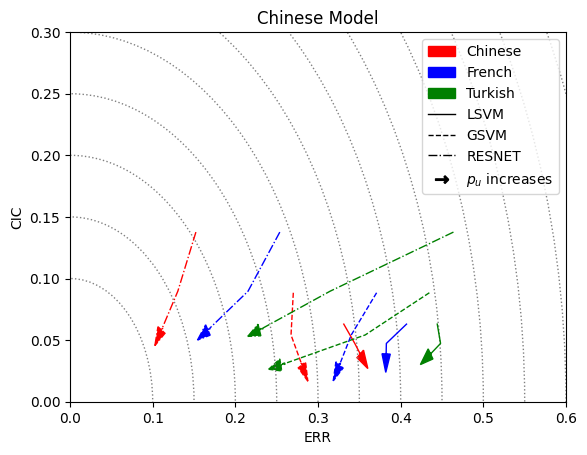
\includegraphics[width=\columnwidth]{Chapter3/FirstPaperFigures/analisi_chinese.png}
\caption{Majority - Chin.}
\end{subfigure} \\
\begin{subfigure}[b]{.55\columnwidth}
\centering
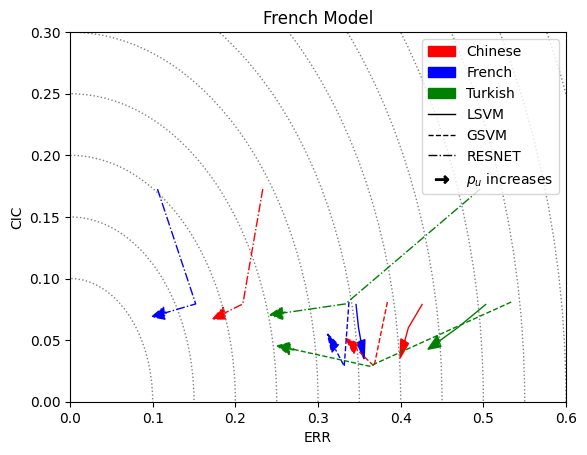
\includegraphics[width=\columnwidth]{Chapter3/FirstPaperFigures/analisi_french.png}
\caption{Majority - Fren}
\end{subfigure} \\
\begin{subfigure}[b]{.55\columnwidth}
\centering
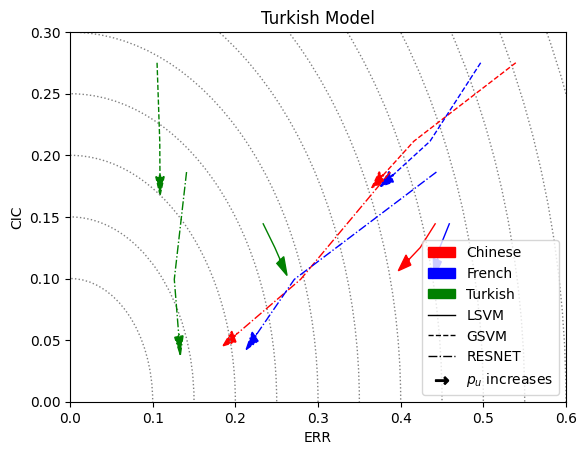
\includegraphics[width=\columnwidth]{Chapter3/FirstPaperFigures/analisi_turkish.png}
\caption{Majority - Turk.}
\end{subfigure} 
\caption{LAMP dataset: graphical representation of Table~\ref{ch3:tab:ris:ml:lamp}. 
x-axis reports the average error on all cultures (ERR) while on the y-axis the CIC varying $p_u$ (arrow indicates the direction of increase of $p_u$) for each algorithm (LSVM, GSVM and RESNET) and for each combination of majority culture and $p_u$ (percentage of minority culture) in the training set and for each possible combination of the cultures (Chin., Fren, and Turk.).}
\label{ch3:fig:ris:ml:lamp}
\end{figure}
%
%
\begin{figure}[H]
\centering
\begin{subfigure}[b]{.55\columnwidth}
\centering
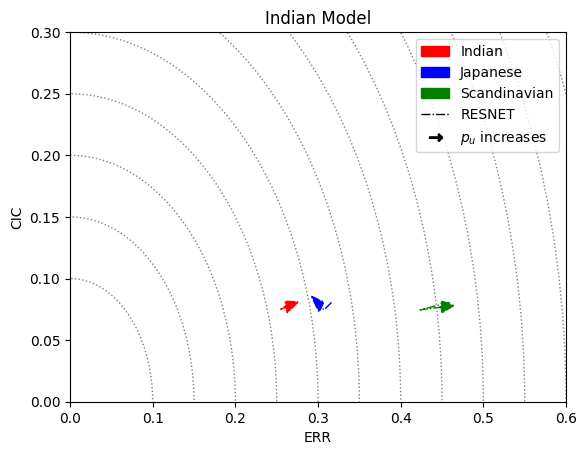
\includegraphics[width=\columnwidth]{Chapter3/FirstPaperFigures/analisi_indian.png}
\caption{Majority - Ind.}
\end{subfigure} \\
\begin{subfigure}[b]{.55\columnwidth}
\centering
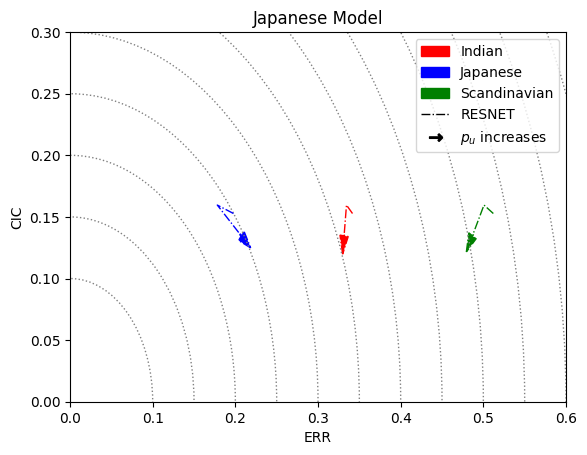
\includegraphics[width=\columnwidth]{Chapter3/FirstPaperFigures/analisi_japanese.png}
\caption{Majority - Japan.}
\end{subfigure} \\
\begin{subfigure}[b]{.55\columnwidth}
\centering
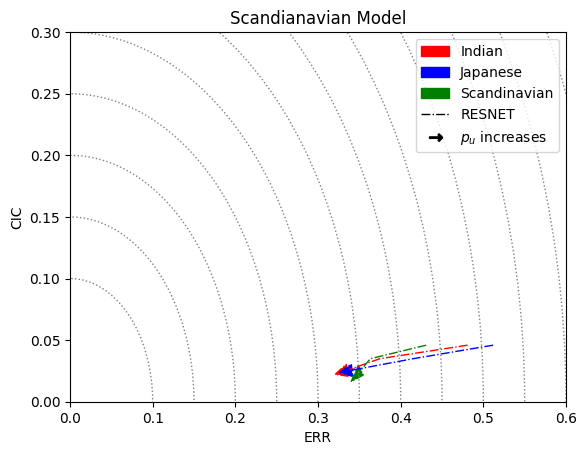
\includegraphics[width=\columnwidth]{Chapter3/FirstPaperFigures/analisi_scandinavian.png}
\caption{Majority - Scand.}
\end{subfigure} 
\caption{CARPET dataset: A graphical representation of Table~\ref{ch3:tab:ris:ml:carpet}. The x-axis shows the average error across all cultures (ERR), while the y-axis represents the CIC varying with $p_u$ (the arrow indicates the direction of increase of $p_u$). This is for the RESNET algorithm and for each combination of majority culture and $p_u$ (percentage of minority culture) in the training set, as well as for each possible combination of the cultures (Ind., Japan., and Scand.).}
\label{ch3:fig:ris:ml:carpet}
\end{figure}
%

\section{Multi-Task-Learning-Inspired Mitigation Strategy}
\label{sec:exp_mitigation:res}
The proposed mitigation framework is applied to the RESNET architecture—identified as the optimal model based on the empirical results delineated in the previous chapter—across both the LAMP and CARPET datasets. 
Evaluations are conducted using minority representation levels $p_u \in \{5\%, 10\%\}$, excluding the $p_u = 0\%$ configuration in accordance with the theoretical constraints established in Section~\ref{ch2:sec:CCML}.
The performance metrics for the MTL interventions are detailed in Tables~\ref{ch3:tab:ris:mtl:lamp} and~\ref{ch3:tab:ris:mtl:carpet}, and further elucidated through the graphical representations in Figures~\ref{ch3:fig:ris:mtl:lamp} and~\ref{ch3:fig:ris:mtl:carpet}.

Table~\ref{ch3:tab:ris:mtl:lamp} details the performance of the mitigated RESNET architecture on the LAMP dataset across each permutation of majority culture and minority representation levels ($p_u \in \{5\%, 10\%\}$). 
The table enumerates the results for varying threshold values $\tau \in \{0, 0.1, 0.2\}$ across all cultural combinations (Chin., Fren, and Turk.).
Specifically, it reports the optimal task-weighting parameter identified during model selection, denoted as $\gamma^*$, the class-specific test error rates ($\text{ERR}^{\text{Chin.}}$, $\text{ERR}^{\text{Fren}}$, and $\text{ERR}^{\text{Turk.}}$), and the resulting CIC. 
Furthermore, to quantify the efficacy of the MTL approach, we provide the percentage improvement ($\%\text{Imp.}$) relative to the non-mitigated baseline configurations established in Section~\ref{ch3:sec:exp_standard_ml} (see Table~\ref{ch3:tab:ris:ml:lamp}).

Table~\ref{ch3:tab:ris:mtl:carpet} provides analogous performance metrics for the CARPET dataset, enabling a direct comparison with the baseline results established in Table~\ref{ch3:tab:ris:ml:carpet}.
To elucidate the impact of the MTL regularizer in mitigating cultural incompetence (as formalized in Section~\ref{ch2:sec:CCML}), Figure~\ref{ch3:fig:ris:mtl:lamp} illustrates the trade-off between the mean error ($\text{ERR}$) on the horizontal axis and the CIC on the vertical axis for the RESNET architecture. 
Each plot corresponds to a specific majority culture at a minority representation level of $p_u=10\%$. 
The trajectories, indicated by directional arrows, signify the evolution of the model as the task-weighting parameter $\gamma$ increases. 
In these visualizations, the arrow color denotes the error rate associated with a specific culture, while the line style (solid, dashed, or dotted) distinguishes between the various algorithmic configurations.

Figure~\ref{ch3:fig:ris:mtl:carpet} is the counterpart of Figure~\ref{ch3:fig:ris:mtl:lamp} for the CARPET dataset.
\begin{table}[H]
\footnotesize
\centering
\setlength{\tabcolsep}{0.1cm}
\renewcommand{\arraystretch}{1.55}
\begin{tabular}{c|c|c|c|c|c|c|}
\toprule
\textbf{Majority} & $\boldsymbol{\tau}$ & $\boldsymbol{\gamma^*}$ & \textbf{ERR$^{\text{Chin.}}$  (\%Imp)}
& \textbf{ERR$^{\text{Fren}}$ (\%Imp)}
& \textbf{ERR$^{\text{Turk.}}$  (\%Imp)}
& \textbf{CIC (\%Imp)} \\
\midrule
\multicolumn{7}{c}{$p_u = 5\%$}\\
\midrule
\multirow{4}{*}{Chin.} & 0.0 & 0.0146 & $11.8\% (\mathbf{-1.2\%})$ & $19.0\% (\mathbf{-2.5\%})$ & $25.1\% (\mathbf{-6.4\%})$ & $7.0\% (\mathbf{-2.0\%})$ \\
& 0.1 & 0.0146 & $11.8\% (\mathbf{-1.2\%})$ & $19.0\% (\mathbf{-2.5\%})$ & $25.1\% (\mathbf{-6.4\%})$ & $7.0\% (\mathbf{-2.0\%})$ \\
& 0.2 & 0.0146 & $11.8\% (\mathbf{-1.2\%})$ & $19.0\% (\mathbf{-2.5\%})$ & $25.1\% (\mathbf{-6.4\%})$ & $7.0\% (\mathbf{-2.0\%})$ \\
\hhline{-------}
\multirow{4}{*}{Fren} & 0.0 & 0.0464 & $18.5\%  (\mathbf{-2.4\%})$ & $9.0\%  (\mathbf{-6.2}\%)$ & $26.0\%  (\mathbf{-7.3}\%)$ & $8.8\% (+0.9\%)$ \\
& 0.1 & 0.0146 & $19.5\%  (\mathbf{-1.4\%})$ & $10.8\%  (\mathbf{-4.4\%})$ & $28.3\%  (\mathbf{-5.0\%})$ & $8.8\%  (+0.9\%)$ \\
& 0.2 & 0.0146 & $19.5\%  (\mathbf{-1.4\%})$ & $10.8\%  (\mathbf{-4.4\%})$ & $28.3\%  (\mathbf{-5.0\%})$ & $8.8\% \ (+0.9\%)$ \\
\hhline{-------}
\multirow{4}{*}{Turk.} & 0.0 & 0.1468 & $25.1\% (\mathbf{-2.8\%})$ & $21.3\% (\mathbf{-5.8\%})$ & $12.1\% (\mathbf{-0.5\%})$ & $7.4\% (\mathbf{-2.5\%})$ \\
& 0.1 & 0.1468 & $25.1\% (\mathbf{-2.8\%})$ & $21.3\% (\mathbf{-5.8\%})$ & $12.1\% (\mathbf{-0.5\%})$ & $7.4\% (\mathbf{-2.5\%})$ \\
& 0.2 & 0.1468 & $25.1\% (\mathbf{-2.8\%})$ & $21.3\% (\mathbf{-5.8\%})$ & $12.1\% (\mathbf{-0.5\%})$ & $7.4\% (\mathbf{-2.5\%})$ \\
\midrule
\multicolumn{7}{c}{$p_u = 10\%$}\\
\midrule
\multirow{3}{*}{Chin.} & 0.0 & 1.0 & $10.6\% (\mathbf{-0.6\%})$ & $13.8\% (\mathbf{-3.1\%})$ & $19.3\% (\mathbf{-4.0\%})$ & $4.1\% (\mathbf{-1.9\%})$ \\
& 0.1 & 0.6813 & $12.4\% (+1.2\%)$ & $13.7\% (\mathbf{-3.2\%})$ & $20.7\% (\mathbf{-2.6\%})$ & $3.8\% (\mathbf{-2.2\%})$ \\
& 0.2 & 0.6813 & $12.4\% (+1.2\%)$ & $13.7\% (\mathbf{-3.2\%})$ & $20.7\% (\mathbf{-2.6\%})$ & $3.8\% (\mathbf{-2.2\%})$ \\
\hhline{-------}
\multirow{3}{*}{Fren} & 0.0 & 0.0146 & $16.8\% (\mathbf{-2.0\%})$ & $9.2\% (\mathbf{-2.4}\%)$ & $20.6\% (\mathbf{-5.5\%})$ & $6.3\% (\mathbf{-0.9\%})$ \\
& 0.1 & 0.04641 & $15.9\% (\mathbf{-2.9\%})$ & $9.4\% (\mathbf{-7.5}\%)$ & $21.5\% (\mathbf{-1.8\%})$ & $6.2\% (\mathbf{-1.0\%})$ \\
& 0.2 & 0.04641 & $15.9\% (\mathbf{-2.9\%})$ & $9.4\% (\mathbf{-7.5}\%)$ & $21.5\% (\mathbf{-1.8\%})$ & $6.2\% (\mathbf{-1.0\%})$ \\
\hhline{-------}
\multirow{3}{*}{Turk.} & 0.0 & 0.0316 & $17.2\% (\mathbf{-3.0\%})$ & $18.0\% (\mathbf{-4.6\%})$ & $10.6\% (\mathbf{-2.5\%})$ & $4.7\% (\mathbf{-0.8\%})$ \\
& 0.1 & 1.578 & $17.8\% (\mathbf{-2.4\%})$ & $18.4\% (\mathbf{-4.2\%})$ & $12.5\% (\mathbf{-0.6\%})$ & $3.7\% (\mathbf{-1.8\%})$ \\
& 0.2 & 1.578 & $17.8\% (\mathbf{-2.4\%})$ & $18.4\% (\mathbf{-4.2\%})$ & $12.5\% (\mathbf{-0.6\%})$ & $3.7\% (\mathbf{-1.8\%})$ \\
\bottomrule
\end{tabular}
\caption{LAMP dataset and the RESNET algorithm: For each combination of majority culture and $p_u$ (percentage of minority culture) in the training set, for different values of $\tau \in {0, 0.1, 0.2}$, and for each possible combination of the cultures (Chin., Fren, and Turk.), the optimal $\gamma$ selected during the model selection phase, denoted as $\gamma^*$, the error on the test set for each culture (ERR$^\text{Chin.}$, ERR$^\text{Fren}$, and ERR$^\text{Turk.}$), and the CIC using our mitigation approach.
Additionally, we report the improvements (\%Imp.) with respect to the non-mitigated scenario described in Section~\ref{ch3:sec:exp_standard_ml}.}
\label{ch3:tab:ris:mtl:lamp}
\end{table}
%
%
\begin{table}[H]
\footnotesize
\centering
\setlength{\tabcolsep}{0.1cm}
\renewcommand{\arraystretch}{1.55}
\begin{tabular}{c|c|c|c|c|c|c|}
\toprule
\textbf{Majority} & $\boldsymbol{\tau}$ & $\boldsymbol{\gamma^*}$ & \textbf{ERR$^{\text{Ind.}}$  (\%Imp)}
& \textbf{ERR$^{\text{Japan.}}$ (\%Imp)}
& \textbf{ERR$^{\text{Scand.}}$  (\%Imp)}
& \textbf{CIC (\%Imp)} \\
\midrule
\multicolumn{7}{c}{$p_u = 5\%$}\\
\midrule
\multirow{3}{*}{Ind.} & 0.0 & 0.06812 & $22.0\% (\mathbf{-3.4\%})$ & $21.6\% (\mathbf{-9.1}\%)$ & $45.6\% (+3.3\%)$ & $9.3\% (+1.8\%)$ \\
& 0.1 & 1.0 & $23.2\% (\mathbf{-2.2\%})$ & $24.3\% (\mathbf{-6.4\%})$ & $44.5\% (+2.2\%)$ & $8.8\%(+1.3\%)$ \\
& 0.2 & 1.0 & $23.2\%(\mathbf{-2.2\%})$ & $24.3\% (\mathbf{-6.4}\%)$ & $44.5\% (+2.2\%)$ & $8.8\% (+1.3\%)$ \\
\hhline{-------}
\multirow{3}{*}{Japan.} & 0.0 & 0.0.01 & $34.6\%(+1.2\%)$ & $17.7\% (\mathbf{-0.1\%})$ & $45.8\%(\mathbf{-4.3\%})$ & $15.0\% (\mathbf{-1.0\%})$ \\
& 0.1 & 0.03162 & $35.7\% (+2.3\%)$ & $21.0\% (+3.2\%)$ & $45.8\% (\mathbf{-4.3\%})$ & $13.1\% (\mathbf{-2.9\%})$ \\
& 0.2 & 0.03162 & $35.7\% (+2.3\%)$ & $21.0\% (+3.2\%)$ & $45.8\% (\mathbf{-4.3\%})$ & $13.1\% (\mathbf{-2.9\%})$ \\
\hhline{-------}
\multirow{3}{*}{Scand.} & 0.0 & 0.04641 & $32.2\% (\mathbf{-5.3\%})$ & $22.1\% (\mathbf{-19.4\%})$ & $38.2\% (+1.9\%)$ & $8.7\% (+5.2\%)$ \\
& 0.1 & 0.0681 & $34.5\% (\mathbf{-3.0\%})$ & $26.8\% (\mathbf{-14.7}\%)$ & $38.8\% (+2.5\%)$ & $6.7\% (+3.2\%)$ \\
& 0.2 & 2.1544 & $33.8\% (\mathbf{-3.7\%})$ & $32.7\% (\mathbf{-8.8\%})$ & $37.1\% (+0.8\%)$ & $5.0\%(+1.5\%)$ \\
\midrule
\multicolumn{7}{c}{$p_u = 10\%$}\\
\midrule
\multirow{3}{*}{Ind.} & 0.0 & 0.2154 & $22.6\% (\mathbf{-3.5\%})$ & $20.2\% (\mathbf{-10.2}\%)$ & $41.9\% (\mathbf{-2.9\%})$ & $8.3\% (+0.6\%)$ \\
& 0.1\%& 0.2154 & $22.6\% (\mathbf{-3.5\%})$ & $20.2\%(\mathbf{-10.2}\%)$ & $41.9\%(\mathbf{-2.9\%})$ & $8.3\% (+0.6\%)$ \\
& 0.2\%& 0.2154 & $22.6\% (\mathbf{-3.5\%})$ & $20.2\% (\mathbf{-10.2}\%)$ & $41.9\% (\mathbf{-2.9\%})$ & $8.3\% (+0.6\%)$ \\
\hhline{-------}
\multirow{3}{*}{Japan.} & 0.0 & 0.1 & $32.3\% (\mathbf{-0.9\%})$ & $18.2\% (\mathbf{-2.4\%})$ & $42.6\% (\mathbf{-6.1}\%)$ & $12.8\% (\mathbf{-0.8\%})$ \\
& 0.1\%& 0.3162 & $34.0\% (+0.8\%)$ & $20.4\% (\mathbf{-0.2\%})$ & $44.1\% (\mathbf{-4.6\%})$ & $12.4\% (\mathbf{-1.2\%})$ \\
& 0.2\%& 0.3162 & $34.0\% (+0.8\%)$ & $20.4\% (\mathbf{-0.2\%})$ & $44.1\% (\mathbf{-4.6\%})$ & $12.4\% (\mathbf{-1.2\%})$ \\
\hhline{-------}
\multirow{3}{*}{Scand.} & 0.0 & 0.0681 & $27.4\% (\mathbf{-6.3}\%)$ & $19.6\% (\mathbf{-14.8}\%)$ & $39.6\% (+4.4\%)$ & $9.3\% (+6.7\%)$ \\
& 0.1\%& 0.01 & $29.8\% (\mathbf{-3.9\%})$ & $24.1\% (\mathbf{-10.3}\%)$ & $39.0\% (+3.8\%)$ & $7.0\% (+4.4\%)$ \\
& 0.2\%& 2.1544 & $33.0\% (\mathbf{-0.7\%})$ & $27.5\% (\mathbf{-6.9}\%)$ & $35.3\% (+0.1\%)$ & $4.5\% (+1.9\%)$ \\
\bottomrule
\end{tabular}
\caption{CARPET dataset and the RESNET algorithm: For each combination of majority culture and $p_u$ (percentage of minority culture) in the training set, for different values of $\tau \in {0, 0.1, 0.2}$, and for each possible combination of the cultures (Ind., Japan. and Scand.), we report the optimal $\gamma$ selected during the model selection phase, namely $\gamma^*$, the error on the test set for each culture (ERR$^\text{Ind.}$, ERR$^\text{Japan.}$, and ERR$^\text{Scand.}$), and the CIC using our mitigation approach. In addition to ERR and CIC, we also report the improvements (\%Imp.) relative to the non-mitigated scenario presented in Section~\ref{ch3:sec:exp_standard_ml}.}
\label{ch3:tab:ris:mtl:carpet}
\end{table}
%
%
\begin{figure}[H]
\centering
\begin{subfigure}[b]{.55\columnwidth}
\centering
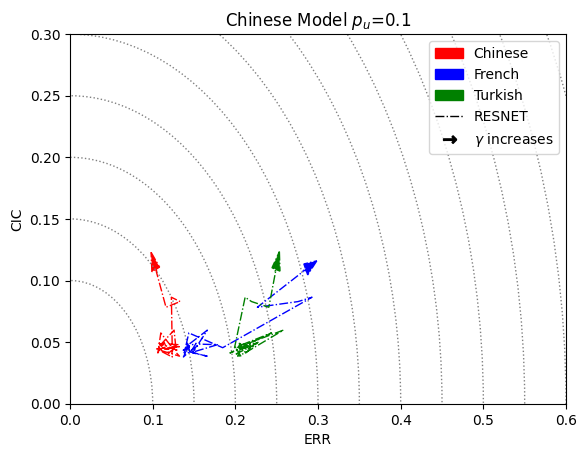
\includegraphics[width=\columnwidth]{Chapter3/FirstPaperFigures/mitigazione_chinese.png}
\caption{Majority - Chin.}
\end{subfigure} \\
\begin{subfigure}[b]{.55\columnwidth}
\centering
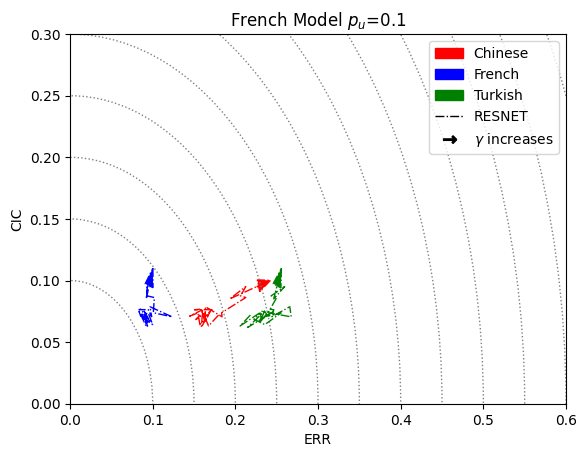
\includegraphics[width=\columnwidth]{Chapter3/FirstPaperFigures/mitigazione_french.png}
\caption{Majority - Fren.}
\end{subfigure} \\
\begin{subfigure}[b]{.55\columnwidth}
\centering
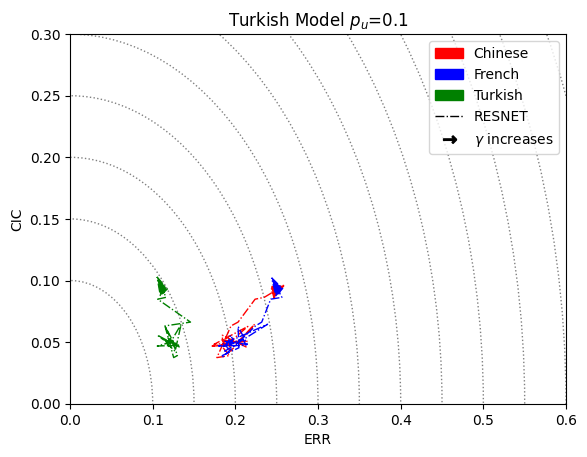
\includegraphics[width=\columnwidth]{Chapter3/FirstPaperFigures/mitigazione_turkish.png}
\caption{Majority - Turk.}
\end{subfigure} 
\caption{LAMP dataset and RESNET algorithm: On the x-axis, we report the average error across all cultures (ERR), while on the y-axis, we report the CIC varying $\gamma$ (with the arrow indicating the direction of increase of $\gamma$), for each combination of majority culture and for each possible combination of the cultures (Chin., Fren, and Turk.) with $p_u = 10\%$.}
\label{ch3:fig:ris:mtl:lamp}
\end{figure}
%
%
\begin{figure}[H]
\centering
\begin{subfigure}[b]{.55\columnwidth}
\centering
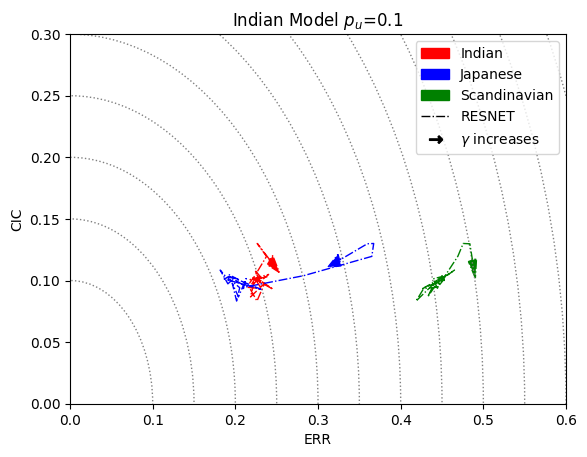
\includegraphics[width=\columnwidth]{Chapter3/FirstPaperFigures/mitigazione_indian.png}
\caption{Majority - Ind.}
\end{subfigure} \\
\begin{subfigure}[b]{.55\columnwidth}
\centering
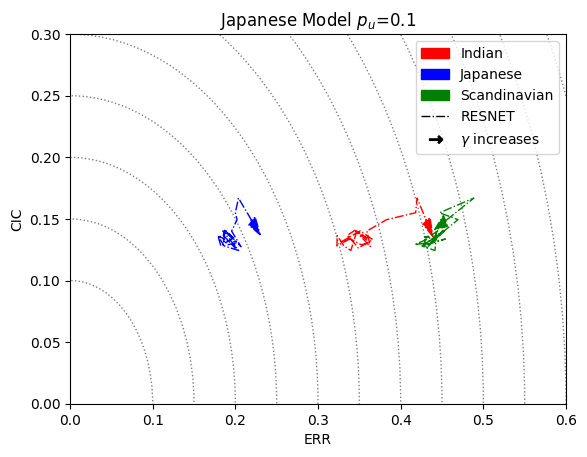
\includegraphics[width=\columnwidth]{Chapter3/FirstPaperFigures/mitigazione_japanese.png}
\caption{Majority - Japan.}
\end{subfigure} \\
\begin{subfigure}[b]{.55\columnwidth}
\centering
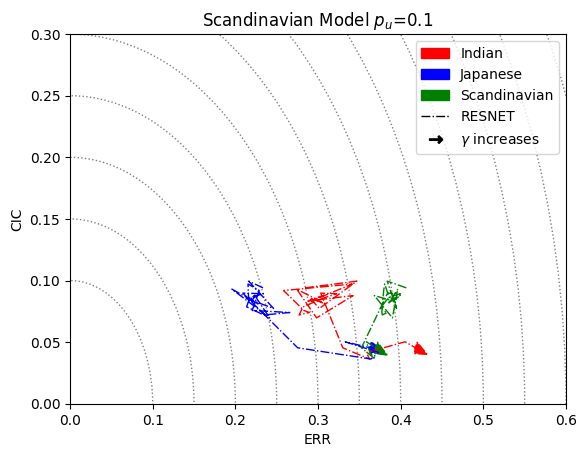
\includegraphics[width=\columnwidth]{Chapter3/FirstPaperFigures/mitigazione_scandianavian.png}
\caption{Majority - Scand.}
\end{subfigure} 
\caption{CARPET dataset and RESNET algorithm: On the x-axis, we report the average error on all cultures (ERR), while on the y-axis, we report the CIC varying $\gamma$ (the arrow indicates the direction of increase of $\gamma$), for each combination of majority culture and each possible combination of the cultures (Ind., Japan., and Scand.) with $p_u = 10\%$.}
\label{ch3:fig:ris:mtl:carpet}
\end{figure}

\section{Conclusion}
This chapter presented a framework for making ML culturally competent. 
The framework is followed by the empirical evaluation of the cultural competence of standard ML algorithms and the effectiveness of the proposed MTL mitigation strategy across the LAMP and CARPET datasets.

The baseline evaluation demonstrated that standard ML algorithms (LSVM, GSVM, and RESNET) are culturally incompetent under conditions of minority under-representation. Across all majority culture permutations and both datasets, the models consistently exhibited lower error rates for the dominant culture while incurring substantially higher error rates for minority cultures, as quantified by the CIC metric. These disparities persisted even as the minority representation level $p_u$ increased, confirming that cultural incompetence is a structural limitation of standard learning algorithms rather than an artifact of extreme data scarcity.

The MTL-inspired mitigation strategy, applied to the RESNET architecture, demonstrated consistent improvements in both class-specific error rates and CIC across the majority of experimental configurations. The task-weighting parameter $\gamma$ proved to be an effective regularization mechanism, enabling the model to balance classification performance and cultural fairness. These results support the theoretical grounding of the proposed framework and indicate that MTL-based mitigation can be applied effectively across diverse cultural contexts and datasets of varying complexity.

Taken together, these findings establish that standard ML algorithms are not culturally competent by default, and that the proposed MTL-inspired mitigation strategy represents a principled and effective approach to reducing cultural bias in object classification tasks.